\documentclass[%
danish,
a4paper,
% onecolumn,
% draftcls
]{report}
\usepackage{EEpreamble}
\usepackage{usecases}
\usepackage{Grp6_tables}

\newcounter{tbr}
\setcounter{tbr}{0}
\newcommand{\tbd}{\textbf{\textcolor{roed}{(TBD)}}}
\newcommand{\tbr}{\textbf{\textcolor{roed}{(TBR)}}}
\usepackage{pdfpages}
\loadglsentries{TeX/Ordliste}

\begin{document}

% Don't fight the engine over float placements. It's actually good at it. If you get ridiculous results it's pretty likely that your paragraphs and/or sections are too short. Try adding more text, or merging some paragraphs.

\newcommand\mymaketitle[1]{
   \rule{\textwidth}{1.6pt}\vspace*{-\baselineskip}\vspace*{2pt}
   \rule{\textwidth}{0.4pt}
   \\   
   {\huge \bf #1}\\
   \rule{\textwidth}{0.4pt}\vspace*{-\baselineskip}\vspace{3.2pt}
   \rule{\textwidth}{1.6pt}
}

\begin{titlepage}
    \begin{center}
        \vspace*{2cm}
        
        % Titel
        \mymaketitle{Robo-Sumo-Battle\\Dokumentationsrapport}
        \vspace{3cm}
        
        % Forfattere
        \large
        \begin{tabular}{ll}
            \multicolumn{2}{c}{\textbf{Gruppe \#6}}\\
            Villiam Holger Bo & 201907166\\
            Adam Ryager Høj & 201803767\\
            Rasmus Kahr & 201803491\\
            David Vestergaard Kristensen & 201908226\\
            Frederik William Lassen & 201905905\\
            Daniel Schultz & 201709325\\
            Simon Fogh Thomsen & 201906472
        \end{tabular}
        \vspace{0.4cm}
        
        % Vejleder
        \textbf{Vejleder:} John Rohde
        \vspace{0.4cm}
        
        % Dato
        \textbf{Dato:} \today
        \vfill
    \end{center}
\end{titlepage}
\tableofcontents
\listoftables
\listoffigures
\clearpage

%% Ordliste
\printglossary[nonumberlist]
\printglossary[type=\acronymtype,nonumberlist,title=Forkortelser]
\clearpage

%% Indledning
\mainpagestyle
\chapter{Indledning}
\section{Koncept}
 Kender vi ikke alle problemet med en drukmås der har drukket for mange øller og får lyst til at skrige i en mikrofon? Det hidtil eneste kendte produkt til at afhjælpe dette problem, har været karaoke, dog med den ulempe at alle andre på baren skal høre på det. Robo-Sumo-Battle vil specifikt afhjælpe dette problem ved i stedet at lade personen bruge sin stemme til at styre to små chubby robotter der dyrker sumo-brydning, som samtidig er sjov at se på - vi bruger således en gammel japansk tradition til at afhjælpe problemerne med en nyere japansk tradition. 

Produktet er et spil for to spillere, hvor hver spiller styrer en to-hjulet robot rundt på en bane.

\figOC{Indledning/RigtBillede.png}{0.8}{Rigt billede der viser hvordan produktet er tiltænkt.}


Styringen foregår via én kontrolenhed pr. spiller og vil være baseret på sensorinput i form af lyd igennem en mikrofon og bevægelse igennem et \textit{d-pad}. Dertil kan man aktivere forskellige \textit{gamemodes} hvor der er udviklet mere eller mindre arbitrære styringer for at skrue sværhedsgraden op. 
Disse signaler bliver digitalt behandlet og sendt til robotterne som styrekommandoer via den embedded software i spilplatformen.
Spillet er tænkt udført som en traditionel japansk sumokamp --- de to robotter mødes i en ring og kæmper. Vinderen er den der fratager alle modstanderens liv først - eller den sidste robot i ringen.

\subsection{Spilregler} \label{Spilregler}

\begin{itemize}
    \item De to robotter anbringes på et markeret \textit{startfelt}.
    \item Når robotterne er anbragt korrekt på deres startfelter, kan en nedtælling fra 3 sekunder startes ved, at begge spillere trykker på hver deres knap, hvorefter spillet går i gang.
    \item Hver robot har fra spillets start 3 liv.
    \item Hver runde vare maksimalt 1 minut.
    \item I en rundes varighed gælder:
    \begin{itemize}
        \item Hvis modstanderen skubbes udover den markerede bane, vindes hele spillet.
        \item Ved at påkøre modstanderen bagfra eller fra siden, mister modstanderen et liv.
        \item Hvis en spiller selv bringer sig udover den markerede bane, vinder modstanderen.
    \end{itemize}
    \item Ved tab af liv placeres hver robot ved deres respektive startfelt.
\end{itemize}

Til styringen af robotterne medfølger der til spillet et instrument med veldefinerede frekvensområder: en blokfløjte. Hertil også et \textit{d-pad}.
\\
 Til disse instrumenter tilknytter der sig som udgangspunkt følgende kommandoer: frem, tilbage, højre og venstre. Disse kommandoer eksekveres med udgangspunkt i \figref{Indledning/blokfloejte_noder} som følgende: 
\begin{itemize}
    \item A: Fremad
    \item B: Bagud
    \item C': Venstre 
    \item D': Højre
\end{itemize}

\fig{Indledning/blokfloejte_noder}{0.2}{Illustration der viser tonaliteten af en blokfløjte. Her ses hvordan styretonerne A, B, C og D spilles}

\fig{Strukturering/Konceptillustrationer/Spilleplade_Topview.eps}{1}{Selve spilpladen}
\fig{Strukturering/Konceptillustrationer/Spilleplade_Sideview.eps}{1}{Spillepladen set fra siden}
\fig{Strukturering/Konceptillustrationer/Spilleplade_Frontview.eps}{1}{Spillepladen set fra den ene spillers side}



%% Krav
\chapter{Krav}

\section{Use Cases}

I det følgende beskrives de use cases der er defineret for systemet, således at de opstillede krav kan opnås. Der er defineret to use cases som fremgår i \figref{Diagrammer/UseCase_Robo-Sumo-Battle}. For de to use cases er der opstillet et sekvensdiagram i \figref{Diagrammer/UseCasesSeqDiag} der beskriver sammenspillet mellem aktørerne for at udføre casen.
Efterfølgende er de to use cases beskrevet på \textit{fully-dressed} form.

\fig{Diagrammer/UCDiagram}{0.6}{Use Case diagram der viser de tre use cases for systemet Robo-Sumo-Battle og aktørernes relation til disse.}
\fig{Diagrammer/UseCasesSeqDiag}{0.8}{Sekvensdiagram der viser samspillet mellem aktørerne for use cases ``Styr SumoBot med joystick'' og ``Styr SumoBot med lyd''.}

%Sometimes it is a good idea to put domain objects in \texttt{}
%The template and the descriptions are based on the book Applying UML and Patterns: 
%An Introduction to Object-Oriented Analysis and Design and Iterative Development
%(3rd Edition) by Craig Larman.

%%% USE CASE 1
\subsubsection{Use Case 1}

Spil \Glspl{rsb} med joystick. Beskrevet i \tabref{usecase:1}.

\begin{usecase}{Fully dressed beskrivelse af Use Case 1: "Spil \gls{rsb} med joystick".}{1}
  \addtitle{Use Case 1}{"Spil \gls{rsb} med joystick"}
  %Level: "user-goal" or "subfunction"
  \addfield{Mål:}{At to spillere, styrer sine respektive \gls{sumobot}, indtil en spiller har vundet}
  %Level: "user-goal" or "subfunction"
  \addfield{Initiering:}{Spillere trykker start på deres respektive start knapper.}

  %Primary Actor: Calls on the system to deliver its services.
  \addfield{Primær Aktør:}{2X Spillere}
  \addfield{Sekundær Aktør:}{Ingen}

  \addfield{Antal samtidig forekomster:}{Ingen}

  %Preconditions: What must be true on start and worth telling the reader?
  \addfield{Prækondition:}{Begge \gls{sumobot} har fuld liv og står på deres respektive startfelter.}
  %when multiple
  %\additemizedfield{Preconditions:}{} 

  %Postconditions: What must be true on successful completion and worth telling the reader
  \additemizedfield{Postkonditioner:}{
    \item En spiller har vundet \gls{rsb} viser vinderen.
    \item \gls{rsb} klar til nyt spil.
  }
  %when multiple
  %\additemizedfield{Preconditions:}{}

  %Main Success Scenario: A typical, unconditional happy path scenario of success.
  \addscenario{Hovedscenarie:}{
    \item Spillere tilgår deres respektive joystick og trykker start.
    \item \gls{rsb} viser nedtælling til start.
    \item Spillere styrer deres respektive \gls{sumobot}s retning og hastighed trådløst via joystick.
    \item Den ene \gls{sumobot} aktivere den anden \gls{sumobot} \gls{AttackSensor}.
    \item[][Udvidelse 1: En \gls{sumobot} forlader spille banen]
    \item \gls{rsb} viser at den angrebet \gls{sumobot} har mistet et liv.
    \item spillere placere deres \gls{sumobot} på dens respektive startfelt og trykker start.
    \item \gls{rsb} viser nedtælling og starter ny runde.
    \item Der spilles til en \gls{sumobot} har mistet alle liv. 
    \item \gls{rsb} viser vinderen af spillet.
    \item Spillere placere \gls{sumobot} på deres respektive startfelter.
    
  }
  \addscenario{Udvidelser / Undtagelser:}{
    \item [Udvidelse 1:] En \gls{sumobot} forlader spillebanen
    \item[1.] \gls{sumobot} der har forladt spillebanen mister alle liv. 
    \item[2.] Use case fortsætter fra punkt 9.
    
  }
\end{usecase}\label{tab:UseCase:1}

%Sometimes it is a good idea to put domain objects in \texttt{}
%The template and the descriptions are based on the book Applying UML and Patterns: 
%An Introduction to Object-Oriented Analysis and Design and Iterative Development
%(3rd Edition) by Craig Larman.

%%% USE CASE 2
\subsubsection{Use Case 2}

Spil \Glspl{rsb} med mikrofon. Beskrevet i \tabref{usecase:2}.

\begin{usecase}{Fully dressed beskrivelse af Use Case 2: "Spil \gls{rsb} med mikrofon".}{2}
  \addtitle{Use Case 2}{"Spil \gls{rsb} med mikrofon"}
  %Level: "user-goal" or "subfunction"
  \addfield{Mål:}{At to spillere, styrer sine respektive \gls{sumobot}, indtil en spiller har vundet}
  %Level: "user-goal" or "subfunction"
  \addfield{Initiering:}{Spillere trykker start på deres respektive start knapper.}

  %Primary Actor: Calls on the system to deliver its services.
  \addfield{Primær Aktør:}{2X Spillere}
  \addfield{Sekundær Aktør:}{Ingen
  }

  \addfield{Antal samtidig forekomster:}{Ingen}

  %Preconditions: What must be true on start and worth telling the reader?
  \addfield{Prækondition:}{Begge \gls{sumobot} har fuld liv og står på deres respektive startfelter.}
  %when multiple
  %\additemizedfield{Preconditions:}{} 

  %Postconditions: What must be true on successful completion and worth telling the reader
  \additemizedfield{Postkonditioner:}{
    \item En spiller har vundet \gls{rsb} viser vinderen.
    \item \gls{rsb} klar til nyt spil.
  }
  %when multiple
  %\additemizedfield{Preconditions:}{}

  %Main Success Scenario: A typical, unconditional happy path scenario of success.
  \addscenario{Hovedscenarie:}{
    \item Spillere tilgår deres respektive mikrofoner og trykker start.
    \item \gls{rsb} viser nedtælling til start.
    \item Spillere styrer deres respektive \gls{sumobot}s retning og hastighed trådløst via påvirke mikrofonen med lyd.
    \item Den ene \gls{sumobot} aktivere den anden \gls{sumobot} \gls{AttackSensor}.
    \item[][Udvidelse 1: En \gls{sumobot} forlader spille banen]
    \item \gls{rsb} viser at den angrebet \gls{sumobot} har mistet et liv.
    \item spillere placere deres \gls{sumobot} på dens respektive startfelt og trykker start.
    \item \gls{rsb} viser nedtælling og starter ny runde.
    \item Der spilles til en \gls{sumobot} har mistet alle liv. 
    \item \gls{rsb} viser vinderen af spillet.
    \item Spillere placere \gls{sumobot} på deres respektive startfelter.
    
  }
  \addscenario{Udvidelser / Undtagelser:}{
    \item [Udvidelse 1:] En \gls{sumobot} forlader spillebanen
    \item[1.] \gls{sumobot} der har forladt spillebanen mister alle liv. 
    \item[2.] Use case fortsætter fra punkt 9.
    
  }
\end{usecase}\label{tab:UseCase:2}



\section{Kravliste} \label{Kravliste}

\subsection{Krav stillet af ASE}
\begin{enumerate}
    \item Systemet \textbf{SKAL} indeholde embedded software.
    \item Systemet \textbf{SKAL} indeholde aktuatorer.
    \item Systemet \textbf{SKAL} indeholde trådløs kommunikation.
    \item Systemet \textbf{SKAL} indeholde et Linux system
    \item Systemet \textbf{SKAL} gøre brug af PSoC
    \item Systemet \textbf{SKAL} gøre brug af sensor(er)
    \item Systemet \textbf{SKAL} indeholde et UI
\end{enumerate}

\subsection{Overordnede krav til Robo-Sumo-Battle}
\begin{enumerate}
    \item Systemet \textbf{SKAL} kunne understøtte minimum 2 spillere.
    \item Systemet \textbf{SKAL} kunne registrer når en SumoBoter overskrider spillebanens afgrænsning.
    \item Systemet \textbf{SKAL} kunne infomere spilleren om spillets status (nedtælling til start, SumoBots restenende liv, resterende spilletid)
    \item Systemet \textbf{BØR} kunne understøtte flere end 2 spillere.  
    \item Systemet \textbf{BØR} understøtte flere spiltilstande, end den allerede beskrevet under spilregler \ref{Spilregler}
\end{enumerate}

\subsection{Spillebane}
\begin{enumerate}
    \item Spillebanen \textbf{SKAL} maximalt være Ø1.5 meter.
    \item Spillebanen \textbf{SKAL} være et jævnt plan.
    \item Spillebanen \textbf{BØR} veje mindre end 10 kg.
\end{enumerate}

\subsection{SumoBot}\label{sumobotkrav}
\begin{enumerate}
    \item SumoBot \textbf{SKAL} maksimalt være $20 \times 20 \times 20$cm.
    \item SumoBot \textbf{SKAL} kunne kollidere med hinanden fra alle sider, ved max hastighed, uden at tage skade.
    \item SumoBot \textbf{SKAL} kunne tilgås trådløst fra minimum tre meters afstand.
    \item SumoBot \textbf{SKAL} veje under 2.5 kg med alt monteret.
    \item SumoBot \textbf {BØR} kunne køre kontinuert, ved max hastighed, vinkelret mod en lodret flade, uden at blive beskadiget.
    \item SumoBot \textbf{BØR} have batterilevetid til kontinueret kørsel ved max hastighed, i minimum 3 minutter.
    \item SumoBot \textbf{BØR} kunne holde til 10cm frit drop på laminatgulv.
    \item SumoBot \textbf{BØR} reagere respektivt på spillerens styring, inden for 1 sekund.
\end{enumerate}


\subsection{Styringsenhed}
    \sisetup{
separate-uncertainty = true,
}
\begin{enumerate}
    \item Styringsenheden \textbf{SKAL} kunne konvertere force på joystick til data som kan omsættes til bevægelse af en \gls{sumobot}'er.
    \item Styringsenheden \textbf{SKAL} have en mikrofon pr. spiller, til at opfange lyd i frekvensområdet \SIrange{300}{3000}{\hertz}.
    \item Styringsenheden \textbf{BØR} have en \ac{SNR} på over \SI{60}{\dB}.
    \item Styringsenheden \textbf{BØR} have en input følsomhed på \SI{8(2)}{\milli\volt\per\pascal}.
    \item Styringsenheden \textbf{BØR} kunne konvertere lyd fra \SIrange{100}{3000}{\hertz} til data som kan benyttes som en del af spillet.
%    \item Styringsenheden \textbf{BØR} ikke påvirkes af lyd under \SI{50}{\dB}.
\end{enumerate}

%% Metode / Proces
\chapter{Proces og metode}
\section{Udviklingsværktøjer}
Rapporten er sat i \LaTeX~med kpfonts.

Desuden er følgende software/hardwareløsninger brugt til at udarbejde \gls{rsb}-projektet.

\subsection{Software}
\begin{itemize}
    \item Overleaf
    \item Mathworks MATLAB R2020a
    \item LTspice XVII
    \item National Instruments Multisim
    \item PlantUML
    \item Microsoft Visio
    \item GitHub
\end{itemize}

Målinger i projektet er foretaget med følgende udstyr, hvoraf noget har været tilgængeligt via. Aarhus Universitets elektroniklaboratorier
\subsection{Måleudstyr}
\begin{itemize}
    \item Analog Discovery 2
    \item Udstyr udlånt af Aarhus Universitet
          \begin{itemize}
              \item KEYSIGHT DSOX20002A Osiloskop
              \item AIM TTi 1604 Multimeter
              \item AIM TTi TG320 Funktionsgenerator
              \item AIM TTi EL302RT Spændingsforsyning
          \end{itemize}
\end{itemize}
% \section{Udviklingsværktøjer}
Rapporten er sat i \LaTeX~med kpfonts.

Desuden er følgende software brugt til at udarbejde \gls{rsb}-projektet.
\subsection{Software}
\begin{itemize}
    \item Overleaf
    \item Mathworks MATLAB R2020a
    \item LTspice XVII
    \item National Instruments Multisim
    \item PlantUML
    \item Microsoft Visio
    \item GitHub
\end{itemize}

Målinger i projektet er foretaget med følgende udstyr, hvoraf noget har været tilgængeligt via. Aarhus Universitets elektroniklaboratorier
\subsection{Måleudstyr}
\begin{itemize}
    \item Analog Discovery 2
    \item Udstyr udlånt af Aarhus Universitet
          \begin{itemize}
              \item KEYSIGHT DSOX20002A Osiloskop
              \item AIM TTi 1604 Multimeter
              \item AIM TTi TG320 Funktionsgenerator
              \item AIM TTi EL302RT Spændingsforsyning
          \end{itemize}
\end{itemize}
\chapter{Risk Assessment}

Arbejdet med risikoanalyse er dels foregået på et overordnet plan hvor potentielle risici for projektet som helhed er identificeret, såvel som et mere blokspecifikt plan, hvor risici for specifikke blokke er identificeret. Disse er naturligvis identificeret med henblik på at minimere disse.

Den egentlige risikoanalyse som ses i \ref{Table:Risk_Assessment} er udarbejdet i forlængelse af struktur-afsnittet hvor de første tanker om analyseafsnittet har været påbegyndt, således at risici er blevet identificeret tidsligt for at kunne forebygge dem tidligst muligt, men ikke tidligere end der eksisterede et overblik over projektet. Det sagt, er identificering af yderligere potentielle risici naturligvist et fortløbende arbejde, ligesom risikominimeringen vil strække sig hele vejen igennem projektet. 


\begin{landscape}
\begin{table}[]
\caption{Risk Assessment}
\label{Table:Risk_Assessment}
\centering
\small
% \begin{tabular}{p{0.1\textwidth}|p{0.3\textwidth}|p{0.05\textwidth}|p{0.05\textwidth}|p{0.05\textwidth}|p{0.3\textwidth}}
\begin{tabular}{
p{0.1\linewidth} % Blok
p{0.25\linewidth} % Desc
p{0.08\linewidth} % Prob.
p{0.09\linewidth} % Cons.
p{0.05\linewidth} % Impact 
p{0.3\linewidth} % Plan
}
\textbf{Blok}& \textbf{Description}& \textbf{Probability} & \textbf{Consequence} & \textbf{Impact} & \textbf{Risk Mitigation Plan}                                                                                                                                                        \\\midrule
Processor        & Vi stiller krav til   processorkraft som ikke kan køre på et embedded system (2xDFT med lille   tidsinterval imellem, wifi, spilstyring mv.) & 2           & 3           & 6      & Krav til processorkraften   overvejes nøje når der vælges processor. Hvis de simultane DFT analyser er en   udfordring overvejes om dette skal foregå på sin egen processor. \\\cmidrule(lr){1-6}
SumoBot IF       & Det lykkedes ikke at overføre   data mellem SumoBot og Central Computer vha. Wifi                                                            & 3           & 5           & 15     & Vi kontakter vejleder og eller   undervisere, der har kendskab til socketprogrammering                                                                                       \\\cmidrule(lr){1-6}
SumoBot IF       & Wifi er for ustabilt til kravet   om konstant overføring af information                                                                      & 1           & 5           & 5      & Vi kontakter vejleder og eller   undervisere, der har kendskab til WiFi                                                                                                      \\\cmidrule(lr){1-6}
Display          & Viser ikke den ønsket   information.                                                                                                         & 2           & 2           & 4      & Spilinformation omlægges til at   vises gennem LED'er                                                                                                                        \\\cmidrule(lr){1-6}
Styrings-enhed IF & Mikrofonens output er for   udefinerbart til at kunne styre en SumoBot med                                                                   & 3           & 4           & 12     & Mikrofonens output analyseres i   blokken "styringsenhed" hvor der er flere resourcer til at omdanne   til et brugbart input                                                 \\\cmidrule(lr){1-6}
Overordnet       & De individuelle delblokke kan   ikke forbindes til et samlet system                                                                          & 3           & 3           & 9      & Delgrupperne i projektgruppen   har løbende kommunikation og tilpasser delblokkende med hinanden.                                                                            \\\cmidrule(lr){1-6}
Overordnet       & Omfanget af SumoBot er for stort   til at kunne nås på den afsatte tid                                                                       & 3           & 3           & 9      & Løbende evaluering og tilretning   af ønsket til endeligt produkt                                                                                                            \\\cmidrule(lr){1-6}
ADC              & Det er ikke muligt at sende data   pga for mange bitfejl                                                                                     & 1           & 5           & 13     & Vi bruger den frivillige øvelse   i MSE på at få indsigt i ADC'er                                                                                                            \\\cmidrule(lr){1-6}
Mikrofon         & Blokfløjtens frekvensspekter er   for snæver til at kunne generere veldefinerede outputs                                                     & 3           & 2           & 6      & Der undersøges andre lydkilder                                                                                                                                               \\\cmidrule(lr){1-6}
PSU              & PSU støjer og transienter   forstyrrer styringsenhed protokollen                                                                             & 3           & 5           & 7      & Vejledere og undervisere med   kendskab til PSU'er kontaktes. Alternativt bruges batteri eller købes/lånes   velfungerende PSU'er                                            \\\cmidrule(lr){1-6}
Overordnet       & Omfanget af spillets realisering   kræver håndværksmæssige kompetencer som vi ikke besidder                                                  & 2           & 5           & 10     & Der søges hjælp på værkstedet i   Shannon eller hos bekendte                                                                                                                 \\\cmidrule(lr){1-6}
Mikrofon         & Støj fra fysiske omstændigheder   (menneskesnak, musik) gør analyse af mikrofon inputtet umuligt                                             & 3           & 5           & 15     & Der søges om rådgivning i   AUDIOlab. Der afsættes tid til at lave akustisk regulering til mikrofon   inputtet.            \\\bottomrule                                                 
\end{tabular}
\end{table}
\end{landscape}

%% Strukturering / Arkitektur !
\chapter{Strukturering}
\section{Robo-Sumo-Battle Strukturering}\label{sec:CC:Strukturering}

For Robo-Sumo-Battle er der udviklet struktur som illustreres ved \figref{Diagrammer/BDD's/OverordnetBDD.png}, og \figref{Strukturering/Robo-Sumo-Battle/IBD_Robo_sumo_battle.pdf}. 
Delblokkene og interfaces imellem disse, som skitseret i IBDet \figref{Strukturering/Robo-Sumo-Battle/IBD_Robo_sumo_battle.pdf} er yderligere beskrevet i blokbeskrivelsen som findes i 
\tabref{blok_table_Robo-Sumo-Battle_blokbeskrivelse}

\fig{Diagrammer/BDD's/OverordnetBDD.png}{0.75}{Robo-Sumo-Battle BDD}
\fig{Strukturering/Robo-Sumo-Battle/IBD_Robo_sumo_battle.pdf}{1}{Robo-Sumo-Battle IBD}



% \begin{SignalDescription}{Robo-Sumo-Battle}{Robo-Sumo-Battle_signalbeskrivelse}
%     \signalbeskrivelse{spillersAntast}{Kraft}{Spillerens fysiske manipulering af joystikket til styring af en SumoBot}
%     \signalbeskrivelse{spillersLyd}{Lyd}{Spillerens fysiske lydinput. Herunder lyd fra fløjte, stemme, mv.}
%     \signalbeskrivelse{Display}{Lys}{Displayets løbende information omkring spilstatus (resterende liv, resterende spilletid mv.)}
%     \signalbeskrivelse{motorDrive}{Torque}{Motorkraften som fysisk får SumoBot til at bevæge sig på banen}
%     \signalbeskrivelse{Styringsprotokol}{SPI}{Digitalt samplet signal af det valgte styringsinput (lyd eller joystick) fra styringsenheden}
%     \signalbeskrivelse{SumoKom}{Wifi}{Tovejskommunikation med SumoBot's hvor der sendes information omkring retning og hastighed og modtage information om et evt. angreb}
%     \signalbeskrivelse{RobotAngreb}{Force}{Et fysisk angreb fra en SumoBot til en anden}
% \end{SignalDescription}



\begin{BlokDescription}{Robo-Sumo-Battle}{Robo-Sumo-Battle_blokbeskrivelse}
%\Blokbeskrivelse{Bloknavn}{Funktion}
%\Portbeskrivelse{Portnavn}{Type}{Beskrivelse}
%%%%%%%%%%%%%%
\Blokbeskrivelse{Styringsenhed}{Omdanner fysisk lyd og joystick påvirkning til data Central Computeren kan læse.}
\Portbeskrivelse{In SpilleresAntast}{Kraft}{Spillerens fysiske manipulering af joysticket}{
\item 
\item 
}
\Portbeskrivelse{In SpillersLyd}{Lyd}{Spillerens fysiske lyd fra stemme eller fløjte}{
\item 
\item 
}
\Portbeskrivelse{Out Styringsprotokol}{SPI}{Digitalt samplet signal af det valgte styringsinput (lyd el-ler joystick) til Central Computer}{
\item 
\item 
}
%%%%%%%%%%%%

\Blokbeskrivelse{Central Computer}{Vidergiver information fra Styringsenhed til Sumobot, trådløst. Informere spillerene om spillets status. Liv, nedtælling etc.}
\Portbeskrivelse{In Styringsprotokol}{SPI}{Digitalt samplet signal af det valgte styringsinput (lyd el-ler joystick) fra styringsenheden}{
\item 
\item 
}
\Portbeskrivelse{Out Display}{Lys}{Displayets løbende information til spillerne omkring spilstatus (re-sterende liv, resterende spilletid mv.)}{
\item 
\item 
}
\Portbeskrivelse{Inout SumoKom}{Wifi}{Tovejskommunikation  med  SumoBot’s  hvor  der  sendesinformation omkring retning og hastighed og modtage in-formation om et evt. angreb}{
\item 
\item 
}
%%%%%%%%%%%%

\Blokbeskrivelse{SumoBot}{Omdanner styringsinfotmation fra Central Computeren, til bevægelse. Informere Centralcomputer om liv er mistet}
\Portbeskrivelse{Inout SumoKom}{Wifi}{Tovejskommunikation  med  Central  Computer  hvor  dermodtages information omkring retning og hastighed ogsendes information om et evt. angreb}{
\item 
\item 
}
\Portbeskrivelse{Inout RobotAngreb}{Force}{}{
\item 
\item 
}
\end{BlokDescription}


\section{Central Computer Strukturering}\label{sec:CC:Strukturering}

For Central Computeren er der udviklet struktur som illustreres ved \figref{Strukturering/Central Computer/CentralComputerBDD.png}, og \figref{Strukturering/Central Computer/IBD_CC.pdf}. 
Delblokkene og interfaces imellem disse, som skitseret i IBDet \figref{Strukturering/Central Computer/IBD_CC.pdf} er yderligere beskrevet i blokbeskrivelsen som findes i 
\tabref{blok_table_Robo-Sumo-Battle_blokbeskrivelse}

\fig{Strukturering/Central Computer/CentralComputerBDD.png}{0.5}{Central Computer BDD}
\fig{Strukturering/Central Computer/IBD_CC.pdf}{1}{Central\_Computer IBD}


% \begin{SignalDescription}{Central Computer}{Central_Computer_signalbeskrivelse}
%     \signalbeskrivelse{Display}{Lys}{Displayets løbende information til spillerne, omkring spilstatus (resterende liv, resterende spilletid mv.)}
%     \signalbeskrivelse{Styringsprotokol}{SPI}{Digitalt samplet signal af det valgte styringsinput (lyd eller joystick) fra styringsenheden}
%     \signalbeskrivelse{SumoKom}{Wifi}{Tovejskommunikation med SumoBot's hvor der sendes information omkring retning og hastighed og modtage information om et evt. angreb}
%     \signalbeskrivelse{displayDataOut}{SPI}{Løbende information omkring spilstatus (re-sterende liv, resterende spilletid mv.)}
% \end{SignalDescription}



\begin{BlokDescription}{Central Computer}{Central_Computer_blokbeskrivelse}
%%%%%%%%%%%%%%
\Blokbeskrivelse{Embedded controller}{Bearbejder og videregiver data fra Styringsenhed til Sumobot, trådløst. sender løbende information  omkring  spilstatus (re-sterende liv, resterende spilletid mv.) til Display blokken}
\Portbeskrivelse{In Styringsprotokol}{SPI}{Digitalt samplet signal af detvalgte styringsinput (lyd eller  joystick)  fra  styringsen-hede}{
\item 
\item 
}
\Portbeskrivelse{Out displayData}{SPI}{Løbende information omkring spilstatus (re-sterende liv, resterende spilletid mv.)}{
\item 
\item 
}
\Portbeskrivelse{Inout SumoKom}{Wifi}{Tovejskommunikation  med  SumoBot’s  hvor  der  sendes information omkring retning og hastighed og modtage in-formation om et evt. angreb}{
\item 
\item 
}
%%%%%%%%%%%%
\Blokbeskrivelse{Display}{Viser løbende information  omkring  spilstatus  (re-sterende liv, resterende spilletid mv.) til spillerne}
\Portbeskrivelse{Out Display}{Lys}{Displayets løbende information til spillerne omkring spilstatus (resterende liv, resterende spilletid mv.)}{
\item 
\item 
}
\Portbeskrivelse{In displayData}{SPI}{Løbende   information   om-kring spilstatus (re-sterendeliv, resterende spilletid mv.)}{
\item 
\item 
}
\BlokSpacer{1.4cm}
\end{BlokDescription}
\section{Styringsenhed Strukturering}\label{sec:Styringsenhed:Strukturering}

For Styringsenheden er der udviklet struktur som illustreres ved \figref{Strukturering/Styringsenhed/XXXXBDDXXXX}, og \figref{Strukturering/Styringsenhed/IBD_styringsenhed}. 
Delblokkene og interfaces imellem disse, som skitseret i IBDet \figref{Strukturering/Styringsenhed/IBD_styringsenhed} er yderligere beskrevet i blokbeskrivelsen som findes i 
\tabref{blok_table_Robo-Sumo-Battle_blokbeskrivelse}

\fig{Strukturering/Styringsenhed/IBD_styringsenhed_rev2}{1}{IBD for Styringsenhed}

\begin{BlokDescription}{Styringsenhed [1/2]}{Styringsenhed_1}
%\Blokbeskrivelse{Bloknavn}{Funktion}
%\Portbeskrivelse{Portnavn}{Type}{Beskrivelse}
\Blokbeskrivelse{Analog signalbehandling}{Forstærker mikrofon inputtet i en grad at ADC kan konvertere de forskellige værdier. \newline Gain: 250gg}
\Portbeskrivelse{Lydsignal}{Analog}{Ufiltreret og forstærket signal indeholdende lydinformation.}{
\item Indgangsimpedans: Høj
}
\Portbeskrivelse{Behandlet lydsignal}{Analog}{Filtreret og forstærket signal indeholdende lydinformation.}{
\item Signalfrekvensområde: \SIrange{300}{3e3}{\Hz}
\item Udgangsimpedans: Lav
}
\BlokSpacer{0cm}
%%%%%%%%%%%%
\Blokbeskrivelse{Mikrofon}{Konvertering fra akustisk til elektrisk signal}
\Portbeskrivelse{Mikrofon}{Analog}{Elektret mikrofon.}{
\item Udgangsimpedans: 2.2\kohm 
\item Sensitivitet: \SI{8(2)}{\milli\volt\per\pascal}
\item SNR: 40dBV
}
\Portbeskrivelse{SpillersLyd}{Akustisk}{Fra mundharmonika.}{
\item Dynamisk område: 70dB SPL
\item Signalfrekvensområde: \SIrange{250}{1550}{\Hz}
}
\Blokbeskrivelse{Signal\newline konditionering}{Buffer stage der skal sikre maksimal spændingsoverførsel.}
\Portbeskrivelse{Behandlet lydsignal}{Analog}{}{
\item Indgangsimpedans: 10x udgangsimpedans for Analog Signalbehandling blokken.
}

\Blokbeskrivelse{ADC}{Analog til digital konvertering.}
\Portbeskrivelse{ADCinLyd}{Analog}{}{
\item Fuld skala input spændingsområde: \SIrange{0}{5}{\volt}
\item Sample rate: 10 kHz.
\item Bitopløsning: 8 bit
\item SNR: 40 dBV
\item Indgangsimpedans: Høj
}

\Blokbeskrivelse{Digital Signal Processing}{Processering af samples fra ADC}
\Portbeskrivelse{DSPin}{Digital}{Array med outputsamples fra ADC}{
\item Type: uint8 (8 bit samples)
\item Antal samples: \tbr
}
\Portbeskrivelse{Styringsprotokol}{SPI}{Retning for SumoBot}{
\item Diskrimineret signalindhold med en frekvensopløsning på 70 Hz til 4 retninger (ligeud, højre, venstre og bagud) for SumoBot.
}
\end{BlokDescription}
\section{SumoBot Strukturering}\label{sec:SumoBot:Strukturering}

For SumoBot er der udviklet struktur som illustreres ved \figref{Strukturering/SumoBot/SumoBot_Bdd.png}, og \figref{Strukturering/SumoBot/IBD_SumoBot.pdf}. 
Delblokkene og interfaces imellem disse, som skitseret i IBDet \figref{Strukturering/SumoBot/IBD_SumoBot.pdf} er yderligere beskrevet i blokbeskrivelsen som findes i 
\tabref{blok_table_Sumobot_blokbeskrivelse_1} og \tabref{blok_table_Sumobot_blokbeskrivelse_2}


\fig{Strukturering/SumoBot/SumoBot_Bdd.png}{1}{SumoBot BDD}

\fig{Strukturering/SumoBot/IBD_SumoBot.pdf}{1}{SumoBot IBD}




\begin{BlokDescription}{Sumobot [1/2]}{Sumobot_blokbeskrivelse_1}
%%%%%%%%%%%% - ATTACK SENCOR
\Blokbeskrivelse{Attack Sensor}{Registrere påkørsel mellem SumoBots. Kollisionsstatus sendes til Microcontroller.}
\Portbeskrivelse{pakoersel}{Force}{Fysisk påvirkning fra omverdenen}{
\item  \SIrange{0}{3.3}{\volt}  signal
}

\Portbeskrivelse{pakoertSignal}{Digital}{Logisk I/O signal}{
\item Spændingsområde: \SIrange{0}{3.3}{\volt}
}
\BlokSpacer{0cm}

%%%%%%%%%%%% - PSU
\Blokbeskrivelse{PSU}{Forsyner de enkelte blokke med korrekt spændingsniveau. Kilden kommer fra batteri.}
\Portbeskrivelse{MCPower}{DC}{Forsyning til Microcontroller}{
\item Spændingsforsyning 5V
}
\Portbeskrivelse{PowerBat}{DC}{Batteri forsyning}{
\item Spændingsniveau: 9V
}
\BlokSpacer{0cm}

%%%%%%%%%%%% - MICROCONTROLLER
\Blokbeskrivelse{Microcontroller}{Styrer motorstyringen ud fra indput fra Central Computer. Ligeledes har MicroControlleren forbindelse med Attack Sensoren og sender dataen videre til Central Computeren.}
\Portbeskrivelse{robotKom}{ SumoBotKom}{WIFI kommunikation fra og til Central Computeren}{
\item trådløs kommunikation mellem Central Computeren og MicroControlleren
}
\Portbeskrivelse{pakoerselRegistrering}{Digital}{Logisk I/O signal fra Attack Sensor}{
\item Spændingsområde: \SIrange{0}{3.3}{\volt}
}
\Portbeskrivelse{motorCmdOutLeft}{Signal}{Signal til motorstyring om venstre motor bestående af 2 logiske signaler og 1 PWM signal}{
\item logisk signal [2] med Spændingsområde: \SIrange{0}{3.3}{\volt}
\item PWM signal med Spændingsområde: \SIrange{0}{3.3}{\volt}
}
\Portbeskrivelse{motorCmdOutRight}{Signal}{Signal til motorstyring om højre motor bestående af 2 logiske signaler og 1 PWM signal}{
\item logisk signal [2] med Spændingsområde: \SIrange{0}{3.3}{\volt}
\item PWM signal med Spændingsområde: \SIrange{0}{3.3}{\volt}
}
\BlokSpacer{0.2cm}
\end{BlokDescription}

\begin{BlokDescription}{Sumobot [2/2]}{Sumobot_blokbeskrivelse_2}

%%%%%%%%%%%% - BATTERI
\Blokbeskrivelse{Batteri}{Forsyner PSU samt motorerne gennem motorstyringen.}
\Portbeskrivelse{chargePowerIn}{DC}{Til batteri fra oplader}{
\item Spændingsniveau: 9V
}
\Portbeskrivelse{PowerBat}{DC}{Fra batteri}{
\item Spændingsniveau: 9V
}
\BlokSpacer{0.4cm}

%%%%%%%%%%%% - MOTOR
\Blokbeskrivelse{Motor}{Skaber fremdrift/bevægelse til Sumobot. Bliver kontrolleret gennem motorstyringen.}
\Portbeskrivelse{motorCtrlIn[2]}{PWM}{PWM fra motorstyring til motor}{
\item PWM signal med Spændingsområde: \SIrange{0}{9}{\volt}
}
\Portbeskrivelse{motorTorqueOut}{torque}{Energi fra motor til hjul}{
\item Moment/energi fra motor til hjul
}
\BlokSpacer{0cm}

%%%%%%%%%%%% - MOTORSTYRING
\Blokbeskrivelse{Motorstyring}{Styrer retning og hastighed af de 2 motorer ud fra kommandoer givet af Microcontrolleren.}
\Portbeskrivelse{motorCommandInRight}{Signal}{Signal til motorstyring om venstre motor bestående af 2 logiske signaler og 1 PWM signal}{
\item logisk signal [2] med Spændingsområde: \SIrange{0}{3.3}{\volt}
\item PWM signal med Spændingsområde: \SIrange{0}{3.3}{\volt}
}
\Portbeskrivelse{motorCommandInLeft}{Signal}{Signal til motorstyring om højre motor bestående af 2 logiske signaler og 1 PWM signal}{
\item logisk signal [2] med Spændingsområde: \SIrange{0}{3.3}{\volt}
\item PWM signal med Spændingsområde: \SIrange{0}{3.3}{\volt}
}
\Portbeskrivelse{motorCtrlOut[2]}{PWM}{PWM signal til motor}{
\item PWM signal med Spændingsområde: \SIrange{0}{9}{\volt} 
}
\end{BlokDescription}



% \section{Projektets mål} 

Projektets overordnede mål tager lige dele udspring i et ønske om et underholdende produkt, som i en grad kan leve videre efter semesterets afslutning såvel som gruppens fælles specifikke teknologiske interesser.
Produktets vision er et konkurrencepræget spil baseret på sumobrydning mellem to robotter i en glasmontre, hvor robotternes retning og hastighed styres på en hidtil ukendte måder – herunder analyse af lydniveauer og frekvenser som produceres af de to spillere såvel som sensorinput af andre arter.
Lyden produceres f.eks. med en blokfløjte eller simpelthen ved stemmens kraft.
Gruppens ønske om undersøgelse af teknologier indenfor analog- og digital lyd behandling indfries naturligt igennem robotternes styringsenheder og ønsket om dybere indsigt i design af software til indlejrede systemer, samt kommunikation mellem disse, indfries igennem hhv. robotterne- og controllernes system- og netværks-design.
Projektet vil yderligere bibringe en stor læring om aktuatorer, mere specifikt motorstyring, som vil være en central del af projektet.

Foruden de faglige mål for læring ønsker gruppen at styrke kendskabet til Scrum som vil anvendes til at styre en iterativ arbejdsproces, som adskiller sig fra processen kendt fra tidligere semestre. 


% \section{Koncept}
 Kender vi ikke alle problemet med en drukmås der har drukket for mange øller og får lyst til at skrige i en mikrofon? Det hidtil eneste kendte produkt til at afhjælpe dette problem, har været karaoke, dog med den ulempe at alle andre på baren skal høre på det. Robo-Sumo-Battle vil specifikt afhjælpe dette problem ved i stedet at lade personen bruge sin stemme til at styre to små chubby robotter der dyrker sumo-brydning, som samtidig er sjov at se på - vi bruger således en gammel japansk tradition til at afhjælpe problemerne med en nyere japansk tradition. 

Produktet er et spil for to spillere, hvor hver spiller styrer en to-hjulet robot rundt på en bane.

Styringen foregår via én kontrolenhed pr. spiller og vil være baseret på sensorinput i form af lyd igennem en mikrofon og bevægelse igennem et \textit{d-pad}. Dertil kan man aktivere forskellige \textit{gamemodes} hvor der er udviklet mere eller mindre arbitrære styringer for at skrue sværhedsgraden op. 
Disse signaler bliver digitalt behandlet og sendt til robotterne som styrekommandoer via den embedded software i spilplatformen.
Spillet er tænkt udført som en traditionel japansk sumokamp --- de to robotter mødes i en ring og kæmper. Vinderen er den robot med flest liv efter endt tid - eller den sidste robot i ringen.

\subsection{Spilregler} \label{Spilregler}

\begin{itemize}
    \item De to robotter anbringes på et markeret \textit{startfelt}.
    \item Når robotterne er anbragt korrekt på deres startfelter, kan en nedtælling fra 3 sekunder startes ved, at begge spillere trykker på hver deres knap, hvorefter spillet går i gang.
    \item Hver robot har fra spillets start 3 liv.
    \item Hver runde vare maksimalt 1 minut.
    \item I en rundes varighed gælder:
    \begin{itemize}
        \item Hvis modstanderen skubbes udover den markerede bane, vindes hele spillet.
        \item Ved at påkøre modstanderen bagfra eller fra siden, mister modstanderen et liv.
        \item Hvis en spiller selv bringer sig udover den markerede bane, vinder modstanderen.
    \end{itemize}
    \item Ved tab af liv placeres hver robot ved deres respektive startfelt.
\end{itemize}

Til styringen af robotterne medfølger der til spillet et instrument med veldefinerede frekvensområder: en blokfløjte. Hertil også et \textit{d-pad}.
\\
 Til disse instrumenter tilknytter der sig som udgangspunkt følgende kommandoer: frem, tilbage, højre og venstre. Disse kommandoer eksekveres med udgangspunkt i \figref{Formalia/blokfloejte_noder} som følgende: 
\begin{itemize}
    \item A: Fremad
    \item B: Bagud
    \item C': Venstre 
    \item D': Højre
\end{itemize}

\fig{Formalia/blokfloejte_noder}{0.6}{}

\fig{Konceptillustrationer/Spilleplade_Topview.eps}{1}{Selve spilpladen}
\fig{Konceptillustrationer/Spilleplade_Sideview.eps}{1}{Spillepladen set fra siden}
\fig{Konceptillustrationer/Spilleplade_Frontview.eps}{1}{Spillepladen set fra den ene spillers side}


% \section{Kravspecifikation for produktet}

\begin{itemize}
    \item Systemet \textbf{SKAL} indeholde embedded software.
    \item Spillebanen \textbf{SKAL} maximalt være Ø1.5 meter.
    \item Robotterne \textbf{SKAL} kunne styres trådløst.
    \item Robotterne \textbf{SKAL} maksimalt være $20 \times 20 \times 20$cm.
    \item Signalbehandling \textbf{SKAL} finde sted. 
    \item Signalbehandling \textbf{BØR} færdiggøres inden for 1 sekund.
    \item Robotterne \textbf{BØR} kunne holde til kollisioner.
    \item Robotterne \textbf{BØR} have batterilevetid til 10 min. aktivitet.
    \item Systemet \textbf{KUNNE} understøtte flere spiltilstande.
    \item Systemet \textbf{KUNNE} understøtte flere spillere.
    \item Robotterne har \textbf{IKKE} våbensystemer.
\end{itemize}
% \clearpage
% \section{Accepttestspecifikation}

\subsection{Krav stillet af ASE}
Se \tabref{ASE Krav}.
\begin{table}[]
\centering
\caption{Krav stillet af ASE}\label{tab:ASE Krav}
\begin{tabular}{c p{7cm}}\toprule
\# & \textbf{Udførsel af test} \\ \midrule
1 & Det konstateres hvorvidt systemet indeholder software indlejret på systemer som ikke er en PC (eksempelvis software på en mikrocontroller)\\\midrule
2 & Det konstateres hvorvidt en systemet gør brug af en aktuator, hvorved der forstås et element som påvirker de fysiske omgivelser, som eksempelvis en DC- eller stepper-motor \\\midrule
3 & Det konstateres hvorvidt systemets fysisk adskilte dele (eksempelvis SumoBot og Bil-kontrol) kommunikerer\\\midrule
4 & Det konstateres hvorvidt minimum et af de indlejrede systemer bruger Linux som styresystem \\\midrule
5 & Det konstateres hvorvidt minimum et PSoC komponent bruges som en del af systemet\\\midrule
6 & Det konstateres hvorvidt systemet optager og benytter data fra komponenter som reagerer på fysisk påvirkning\\\bottomrule
\end{tabular}
\end{table}

\subsection{Overordnede krav til til Robo-Sumo-Battle}

\begin{table}[]
\centering
\caption{Overordnede krav}\label{tab:Overordnede krav}
\begin{tabular}{c p{7cm}}
\# & \textbf{Udførsel af test} \\ \toprule
1 & Det konstateres hvorvidt systemet understøtter minimum 2 spillere. Ved det forstås at der er minimum 2 controllerenheder som styrer hver sin SumoBot, såvel som at pointsystemet kan tælle point for minimum 2 spillere \\\midrule
2 & Gameplay-modulet implementeres således at det visuelt kan identificeres når en SumoBot overskrider spilbanens kant. Herefter styres alle SumoBots som er en del af systemet, ud over spilkantens afgrænsning (4 vilkårlige steder, så langt fra hinanden som muligt), og det bekræftes at systemet har opfattes deres overskridelse af spillebanens kant på baggrund af den visuelle idenficiering. \\\midrule
3 & Ved understøttelse af mere end to spillere slækkes accepttesten til at indbefatte at mere end én spiller, på hver af 2 hold, kan deltage aktivt i styringen af det respektive holds SumoBot. Det konstateres hvorvidt dette er muligt som en naturlig del af spillet\\\midrule
4 & En spiltilstand defineres som en måde at spille på, med hvert sit særlige mål. Det konstateres om der er beskrevet mere end én måde at spille på og der gennemføres et spil af hver spiltilstand. \\\bottomrule
\end{tabular}
\end{table}

\subsection{Krav til controllerne}

\begin{table}[]
\centering
\caption{Krav til controlleren}\label{tab:Controller Krav}
\begin{tabular}{c p{7cm}}
\# & \textbf{Udførsel af test} \\ \midrule
1 & Joystikket flyttes fremad og det konstateres hvorvidt SumoBot bevæger sig fremad. Det samme udføres for bagud, venstre og højre  \\\midrule
2 & Der udarbejdes særskilt testsoftware som på en PC kan gengive det dominerende frekvensindhold i spektret 300Hz - 3000Hz. Herefter testes om frekvenserne 300Hz, 400Hz, 500Hz, 1200Hz, 1800Hz, 2500Hz, 2800Hz, 2900Hz, 3000Hz genkendes. Frekvenserne dannes som sinusbølger og afspilles ved 75dB +/- 5 dB, 20 cm. fra controllerens mikrofon. \\\midrule
3 & Der udarbejdes særskilt testsoftware som på en PC kan gengive det dominerende frekvensindhold i spektret 300Hz - 3000Hz. Dette testsoftware kan også indikere om amplituden er høj nok til at spillet bør reagere på det. Der testes med lyd som afspiller 20 cm fra controllerens mikrofon på hhv. 30 dB, 35 dB, 40 dB, 45 dB, 50 dB, 55 dB, 60 dB. For værdier >50 dB forventes indikation fra softwaren om at der ingen tilstrækkeligt høje lyde er.\\\bottomrule
\end{tabular}
\end{table}

\subsection{Krav til spillebane}

\begin{table}[]
\centering
\caption{Krav til Spillebanen}\label{tab:ASE Krav}
\begin{tabular}{c p{7cm}}
\# & \textbf{Udførsel af test} \\ \midrule
1 & Da spillebanen er rund laves der et stykke snor på 75 cm. Den ene ende af snoren placeres i centrum af spillebanen, mens den anden ende føres langs kanten af spillebanen. Der noteres om snorens ende på noget tidspunkt er kortere end spillebanens kant. \\\midrule
2 & Spille banen placeres på en overflade i vatter. Der findes et vatterpas mellem 1.3 og 1.5 meter. Dette placeres i midten af spillebanen og drejes hele vejen rundt om centrum. Der noteres om spillepladen på noget tidspunkt er ude af vatter.  \\\midrule

3 &  Der findes en kalibreret vægt, med målenøjagtighed på +/- 200g. Alle spillets bestanddele placeres samlet på vægten. den viste vægt noteres\\\midrule

\end{tabular}
\end{table}

\subsection{Krav til robotterne}

\begin{table}[]
\centering
\caption{Krav til Robotterne}\label{tab:ASE Krav}
\begin{tabular}{c p{7cm}}
\# & Udførsel af test \\ \midrule
1 & Der tegnes en 20 x 20 cm kvadratisk firkant på et stykke papir. Herefter placeres robotterne i firkanten, hvor der ses om de stikker ud over kanterne. Herefter måles højden af robotterne med en tommestok hvor der noteres om robotterne er højere end 20 cm. \\\midrule
2 & Der laves en bane på gulvet med tape på 1.5 Meter. Herefter placeres de 2 robotter, fuld opladt, i hver sin ende af banen. Der udføres 4 tests hvor den ene robot med Maks hastighed køre den fulde banes længde inden den rammer den anden robot som holder stille i den anden ende af banen. For hver test vil den stillestående robot blive roteret 90 grader. Efter testen noteres der om der er kommet skader på nogle af bilerne. Og det hele gentages hvor robotterne bytter roller. \\\midrule
3 & Der opmåles en 3 meters strækning med målebånd på gulvet. Robotten startes med fuld opladt batteri og køres ved Maks hastighed i 1 minut. Herefter placeres robotten med fronten væk fra banen i den ene ende af den 3 meter strækning opmålt, mens senderen placeres i den anden ende. Herefter noteres der om det er muligt for robotten at modtage en kommando om at køre fremad væk fra senderen. Dette gentages for den anden robot \\\midrule
4 & Robotterne placeres, fuld opladt, vandret med fronten mod en lodret 90 graders flade, på minimum 30*30 cm. f.eks. gulv og væg. Herefter sættes robotterne til at køre med Maks hastighed fremad for 1 minut mens strømmen gennem motorene måles. SumoBot må ikke ændre placering under testen. Der noteres om strømmen overskrider hvad databladet angiver som max.
\\\midrule
5 & Robotten placeres, fuld opladt, på gulvet, hvor den vil med Maks hastighed køre fremad for 3 minutter. Dette gentages for den anden robot og der noteres om den stopper før de 3 minutter er gået. \\\midrule
6 & Der opmåles 10.cm på en væg fra laminatgulvet, og markeres med f.eks. tape. Herefter tages robotterne og anbringes med deres laveste punkt over den opmålte højde, og lader dem falde i frit fald ned på laminatgulvet. Robotterne skal være fuld funktionelle efter testen.  \\\midrule
7 & Robotten anbringes, fuld opladt, på gulvet, og kører herefter med Maks hastighed for 1 minut. Robotten anbringes herefter inden for 3 meter af senderen. Der optages en video på 30 FPS, af en spiller der anvender controlleren til at henholdsvis køre frem, tilbage, og til siderne med 4 sekunders mellemrum. Herefter anvendes FPS i videoen til at udregne reaktionstiden fra brugeren anvender kontrolleren til robotten reagerer på kommandoen. \\\midrule

\end{tabular}
\end{table}

% \section{Blokdiagrammer}
\section{Overordnet system blokdiagram}

\fig{Diagrammer/SystemBDD}{0.6}{Overordnet systemdiagram}

\fig{Diagrammer/SystemFlow}{0.8}{Overordnet systemdiagram}
\subsection{Bilkontrol}


\subsubsection*{\textbf{Bilkontrol}}
Bilkontrollen er den centrale enhed som samler input fra controllere, sender signal til de to bots om retning og hastighed og styrer spillet. 
\subsubsection*{\textbf{Embedded controller}}
Bilkontrollens software eksekveres på en embedded controller med Linux-system. 
\subsubsection*{\textbf{Receiver}}
Receiver-modulet modtager serielt ikke-processeret input fra controllerens joystik og mikrofon via kabel. 
\subsubsection*{\textbf{Transmitter}}
Transmitter-modulet varetager den trådløse forbindelse til de to bots.
\subsubsection*{\textbf{Trådløs IF}}
Trådløse interface-modulet fungerer som undermodul til Transmitter-modulet og varetager den trådløse forbindelse til de to bots. 
\subsubsection*{\textbf{Digital lydbehandling}}
Digital lydbehandlings-modulet processerer mikrofonernes inputs således disse kan indgå i gameplayet som en styring til de to bots.  
\subsubsection*{\textbf{Gameplay}}
Gameplay-modulet varetager styring af spillets gang mv.  
\subsubsection*{\textbf{Point}}
Point-undermodulet til gameplay-modulet styrer spillernes point 
\subsubsection*{\textbf{Display}}
Display-undermodulet til gameplay-modulet viser kampens status igennem spillernes point. 
\subsubsection*{\textbf{Controller behandling}}
Controller behandlingsmodulet omsætter de ikke-processerede input fra controlleren (herved forstås input fra joystik og mikrofon) og omsætter dem til retning og hastighed for de to bots.  
\subsubsection*{\textbf{Joystick behandling}}
Joystick behandlingsmodulet omsætter det ikke-processerede input fra joystikket til retning og hastighed for de to bots.

\begin{figure*}
	\centering
   	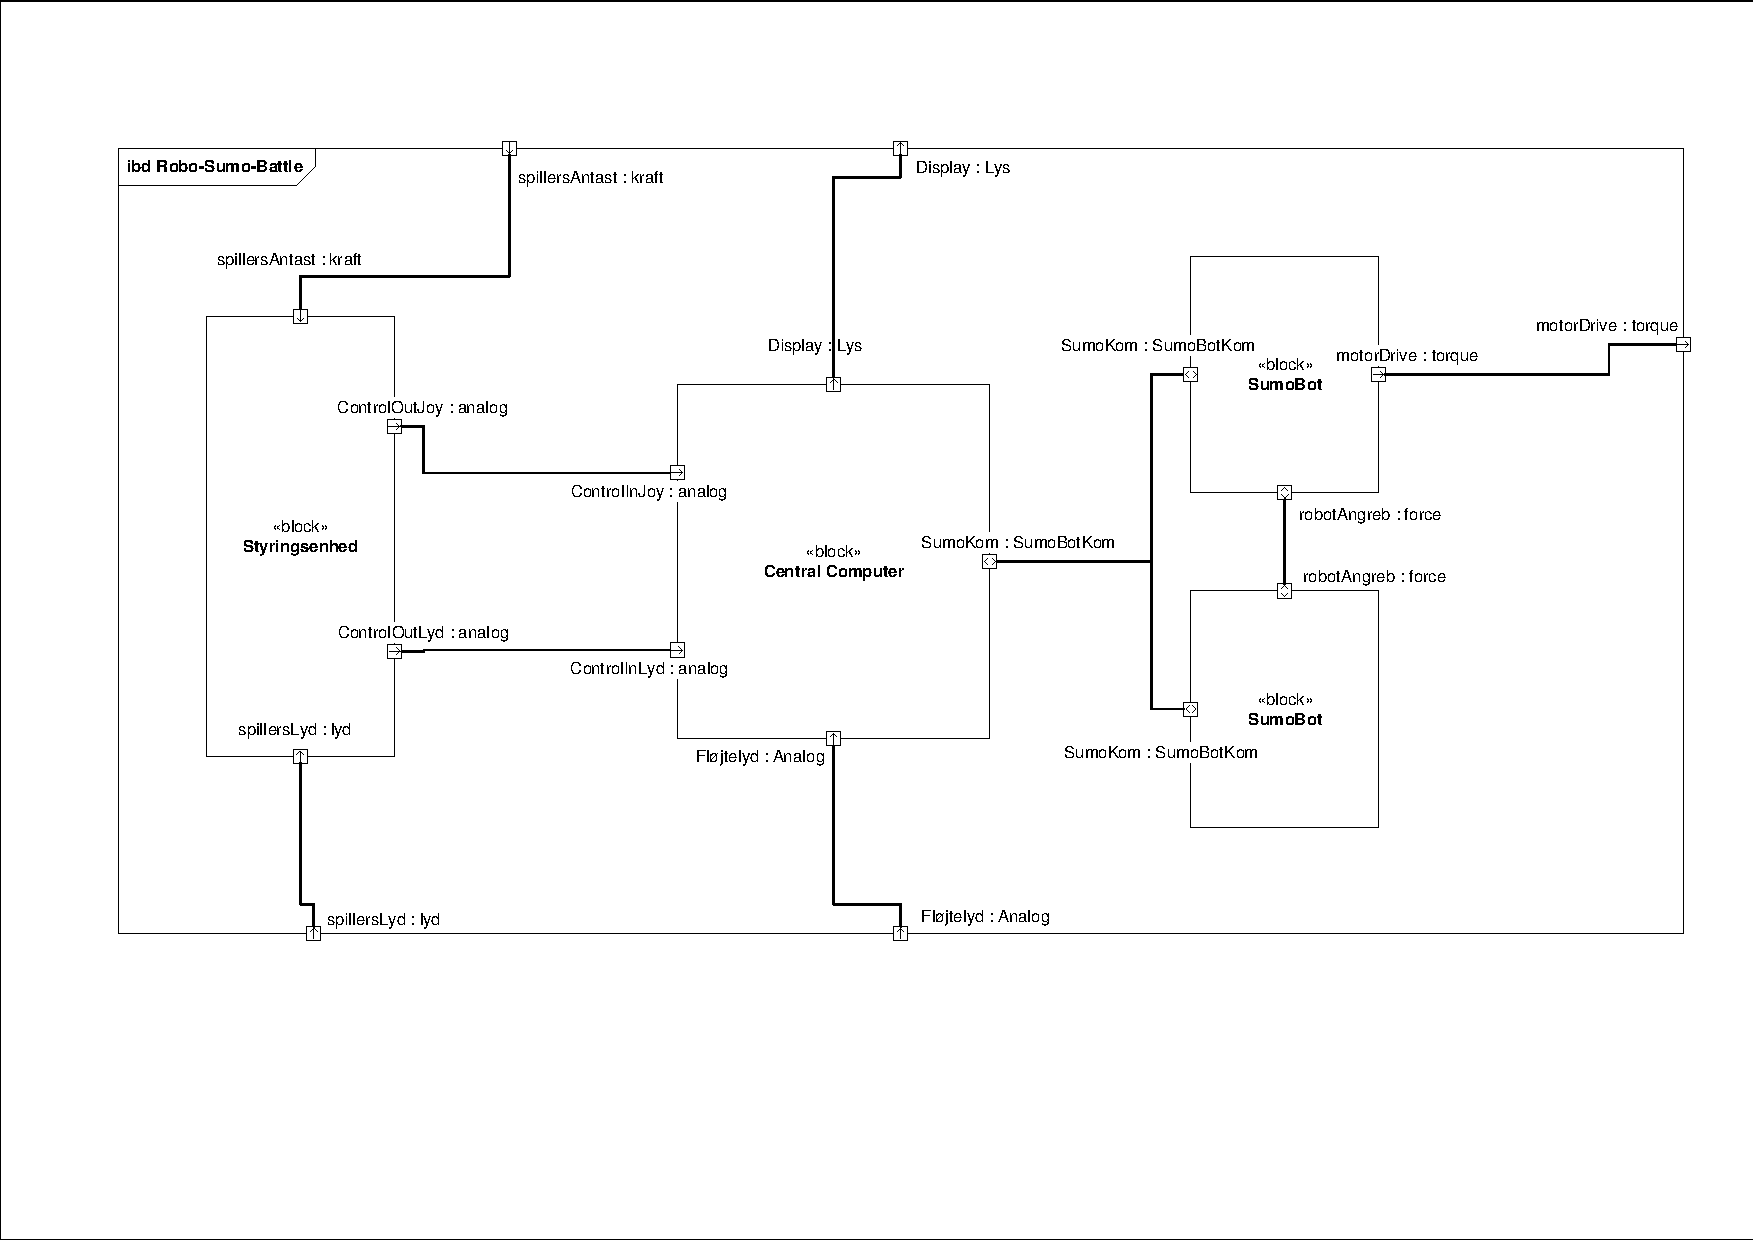
\includegraphics[page=1,width=1\linewidth]{figs/Diagrammer/IBD.pdf}
	\caption{System IBD}
	\label{fig:IBD_System}
\end{figure*}
\begin{figure*}
	\centering
   	\includegraphics[page=2,width=1\linewidth]{figs/Diagrammer/IBD.pdf}
	\caption{IBD for Styringsenhed}
	\label{fig:IBD_Styringsenhed}
\end{figure*}
\begin{figure*}
	\centering
   	\includegraphics[page=3,width=1\linewidth]{figs/Diagrammer/IBD.pdf}
	\caption{IBD for Central Computer}
	\label{fig:IBD_CentralComputer}
\end{figure*}

\begin{figure*}
	\centering
   	\includegraphics[page=4,width=1\linewidth]{figs/Diagrammer/IBD.pdf}
	\caption{IBD for SumoBot}
	\label{fig:IBD_SumoBot}
\end{figure*}

\subsection{Kontroller}
\subsubsection*{\textbf{Controller}}\hfill\\
Controller udgøre grænsefladen til den fysiske værden. Her konvertere force og lyd til data som bilkontrol kan læse og respondere på.
\subsubsection*{\textbf{Microcontroller}}\hfill\\
Microcontroller står for alt modtagelse af analoge signaler fra henholdsvis lydmodul og Joystick, oversætter det til data, som derfra sendes til Bilkontrold via transmitteren.
\subsubsection*{\textbf{Transmitter}}\hfill\\
Kommunikations portal til bilkontrol.
\subsubsection*{\textbf{ADC}}\hfill\\
Oversætter analoge signaler til digitale.
\subsubsection*{\textbf{Joystick}}\hfill\\
Joystic oversætter force til spændinger, som kan læses af microcontrolleren.
\subsubsection*{\textbf{Lyd-modul}}\hfill\\
Lydmodul konvertere lyd til analoge signaler som microcontrolleren kan evaluere på.
\subsubsection*{\textbf{Mikrofon}}\hfill\\
mikrofon gør det muligt for systemet at modtage lyd fra omverdenen.
\subsubsection*{\textbf{Analog filterbehandling}}\hfill\\
Analog filterbehandling filtrerer uønsket frekvenser modtaget fra mikrokrofonen og forstærker eller formindsker signalet, således det er læsbart for en mikrocontroller.



\subsection{Robot}

\figOC{Diagrammer/SumoBot_Bdd.png}{0.6}{System Blokdiagram over sumobot}

\subsubsection*{\textbf{Batteri}}\hfill\\
Forsyner vores system
\subsubsection*{\textbf{Motorstyring}}\hfill\\
Kontrollerer hastighed (vha. PWM) og rotationsretning via H-bro. Bliver styret af PSoC
\subsubsection*{\textbf{Motor}}\hfill\\
En DC-motor der roterer hjul efter en given hastighed og retning fra motorstyring
\subsubsection*{\textbf{PSU}}\hfill\\
Forsyner korrekt spænding til de enkelte delelementer i systemet
\subsubsection*{\textbf{RPi}}\hfill\\
Ansvarlig for den trådløse kommunikation mellem controller og PSoC.
\subsubsection*{\textbf{PSoC}}\hfill\\
Hovedstyringen for SumoBot. \\
Styrer motorstyring afhængig af signal fra RPI’en
Derudover modtager input fra attacksensor, der bearbejder disse til indikering af liv (afventer videre detaljer omkring spilregler)
\subsubsection*{\textbf{AttackSencor}}\hfill\\
Registrering af ”angreb”, som gives videre til PSoC.
\subsubsection*{\textbf{Scoreboard}}\hfill\\
En visuel indikering til brugeren af antal liv for de enkelte SumoBots

% \subsection{Bilkontrol}


\subsubsection*{\textbf{Bilkontrol}}
Bilkontrollen er den centrale enhed som samler input fra controllere, sender signal til de to bots om retning og hastighed og styrer spillet. 
\subsubsection*{\textbf{Embedded controller}}
Bilkontrollens software eksekveres på en embedded controller med Linux-system. 
\subsubsection*{\textbf{Receiver}}
Receiver-modulet modtager serielt ikke-processeret input fra controllerens joystik og mikrofon via kabel. 
\subsubsection*{\textbf{Transmitter}}
Transmitter-modulet varetager den trådløse forbindelse til de to bots.
\subsubsection*{\textbf{Trådløs IF}}
Trådløse interface-modulet fungerer som undermodul til Transmitter-modulet og varetager den trådløse forbindelse til de to bots. 
\subsubsection*{\textbf{Digital lydbehandling}}
Digital lydbehandlings-modulet processerer mikrofonernes inputs således disse kan indgå i gameplayet som en styring til de to bots.  
\subsubsection*{\textbf{Gameplay}}
Gameplay-modulet varetager styring af spillets gang mv.  
\subsubsection*{\textbf{Point}}
Point-undermodulet til gameplay-modulet styrer spillernes point 
\subsubsection*{\textbf{Display}}
Display-undermodulet til gameplay-modulet viser kampens status igennem spillernes point. 
\subsubsection*{\textbf{Controller behandling}}
Controller behandlingsmodulet omsætter de ikke-processerede input fra controlleren (herved forstås input fra joystik og mikrofon) og omsætter dem til retning og hastighed for de to bots.  
\subsubsection*{\textbf{Joystick behandling}}
Joystick behandlingsmodulet omsætter det ikke-processerede input fra joystikket til retning og hastighed for de to bots.

\begin{figure*}
	\centering
   	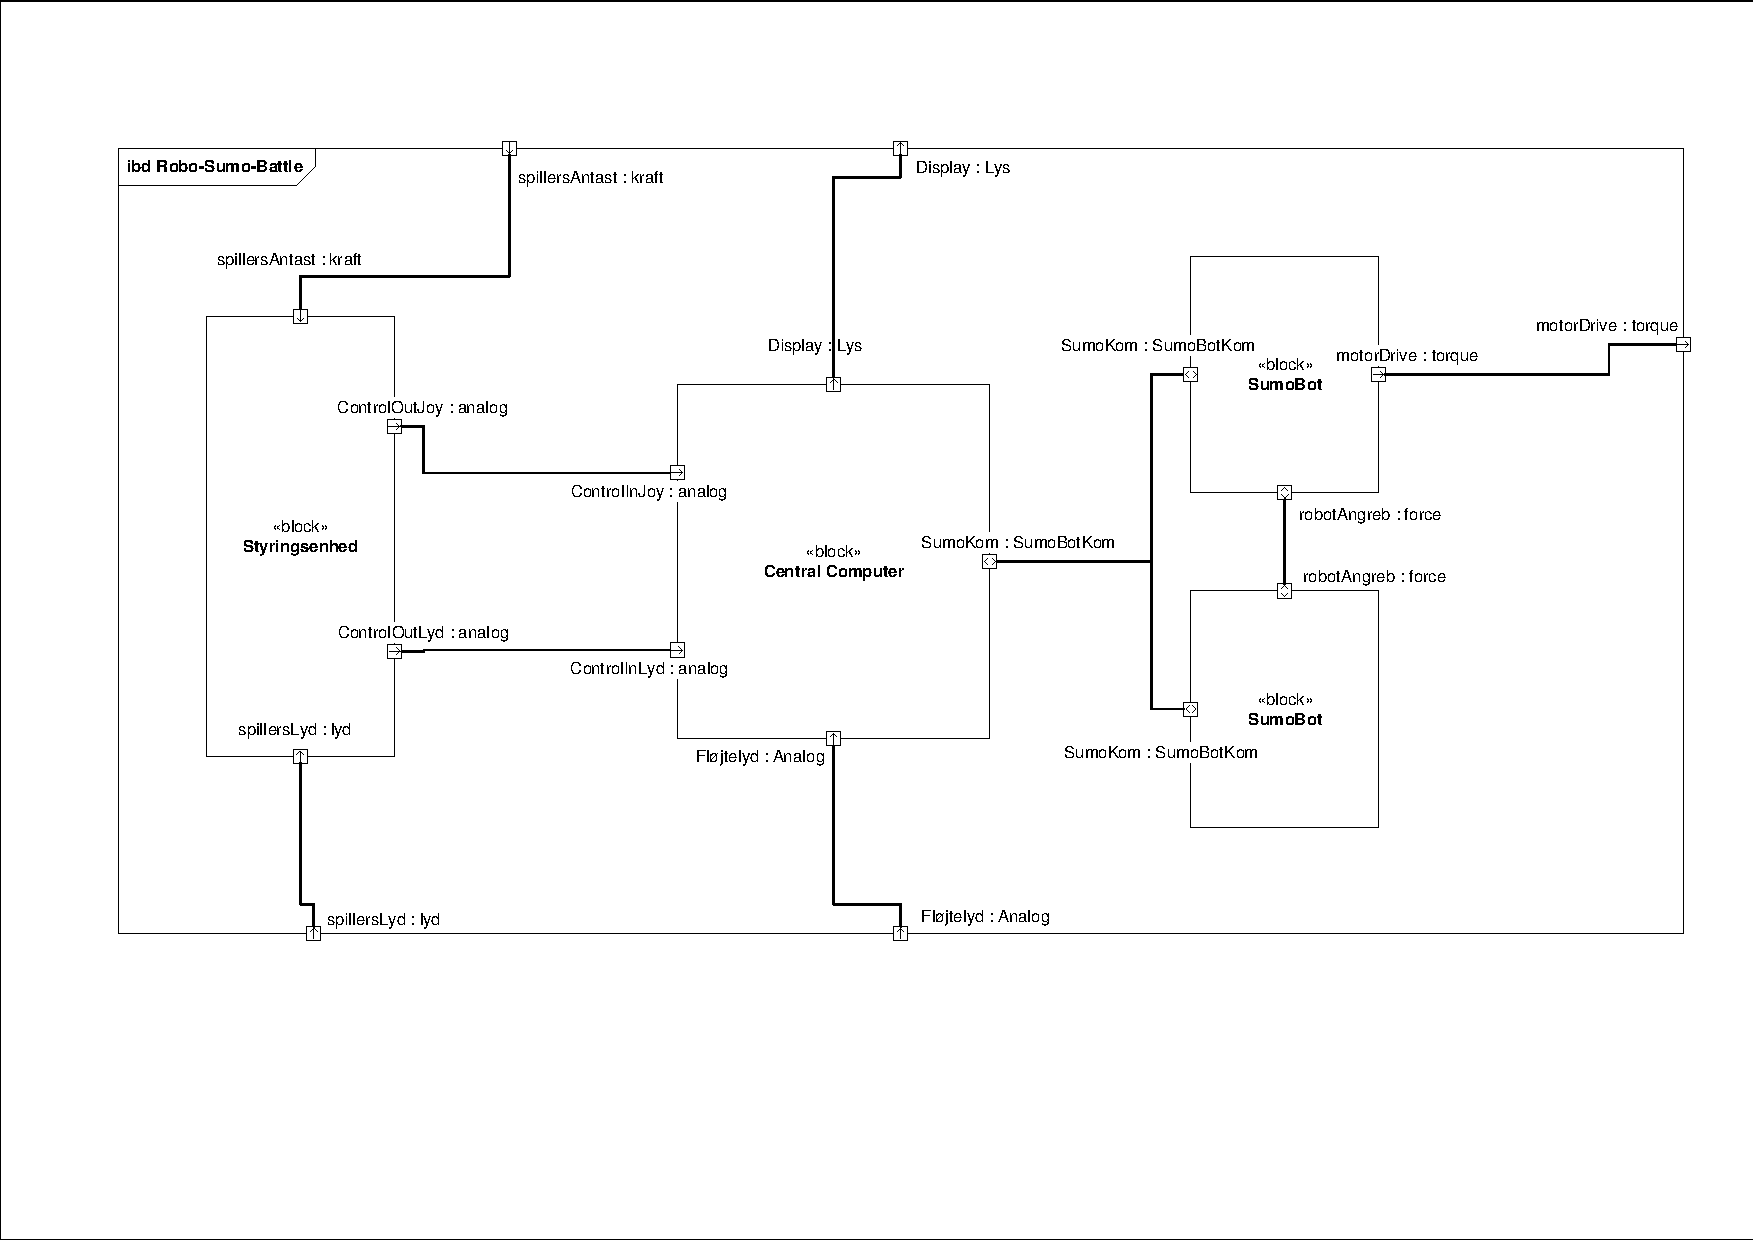
\includegraphics[page=1,width=1\linewidth]{figs/Diagrammer/IBD.pdf}
	\caption{System IBD}
	\label{fig:IBD_System}
\end{figure*}
\begin{figure*}
	\centering
   	\includegraphics[page=2,width=1\linewidth]{figs/Diagrammer/IBD.pdf}
	\caption{IBD for Styringsenhed}
	\label{fig:IBD_Styringsenhed}
\end{figure*}
\begin{figure*}
	\centering
   	\includegraphics[page=3,width=1\linewidth]{figs/Diagrammer/IBD.pdf}
	\caption{IBD for Central Computer}
	\label{fig:IBD_CentralComputer}
\end{figure*}

\begin{figure*}
	\centering
   	\includegraphics[page=4,width=1\linewidth]{figs/Diagrammer/IBD.pdf}
	\caption{IBD for SumoBot}
	\label{fig:IBD_SumoBot}
\end{figure*}

\subsection{Kontroller}
\subsubsection*{\textbf{Controller}}\hfill\\
Controller udgøre grænsefladen til den fysiske værden. Her konvertere force og lyd til data som bilkontrol kan læse og respondere på.
\subsubsection*{\textbf{Microcontroller}}\hfill\\
Microcontroller står for alt modtagelse af analoge signaler fra henholdsvis lydmodul og Joystick, oversætter det til data, som derfra sendes til Bilkontrold via transmitteren.
\subsubsection*{\textbf{Transmitter}}\hfill\\
Kommunikations portal til bilkontrol.
\subsubsection*{\textbf{ADC}}\hfill\\
Oversætter analoge signaler til digitale.
\subsubsection*{\textbf{Joystick}}\hfill\\
Joystic oversætter force til spændinger, som kan læses af microcontrolleren.
\subsubsection*{\textbf{Lyd-modul}}\hfill\\
Lydmodul konvertere lyd til analoge signaler som microcontrolleren kan evaluere på.
\subsubsection*{\textbf{Mikrofon}}\hfill\\
mikrofon gør det muligt for systemet at modtage lyd fra omverdenen.
\subsubsection*{\textbf{Analog filterbehandling}}\hfill\\
Analog filterbehandling filtrerer uønsket frekvenser modtaget fra mikrokrofonen og forstærker eller formindsker signalet, således det er læsbart for en mikrocontroller.



% \section{Interne blokdiagrammer}
\begin{figure*}
	\centering
   	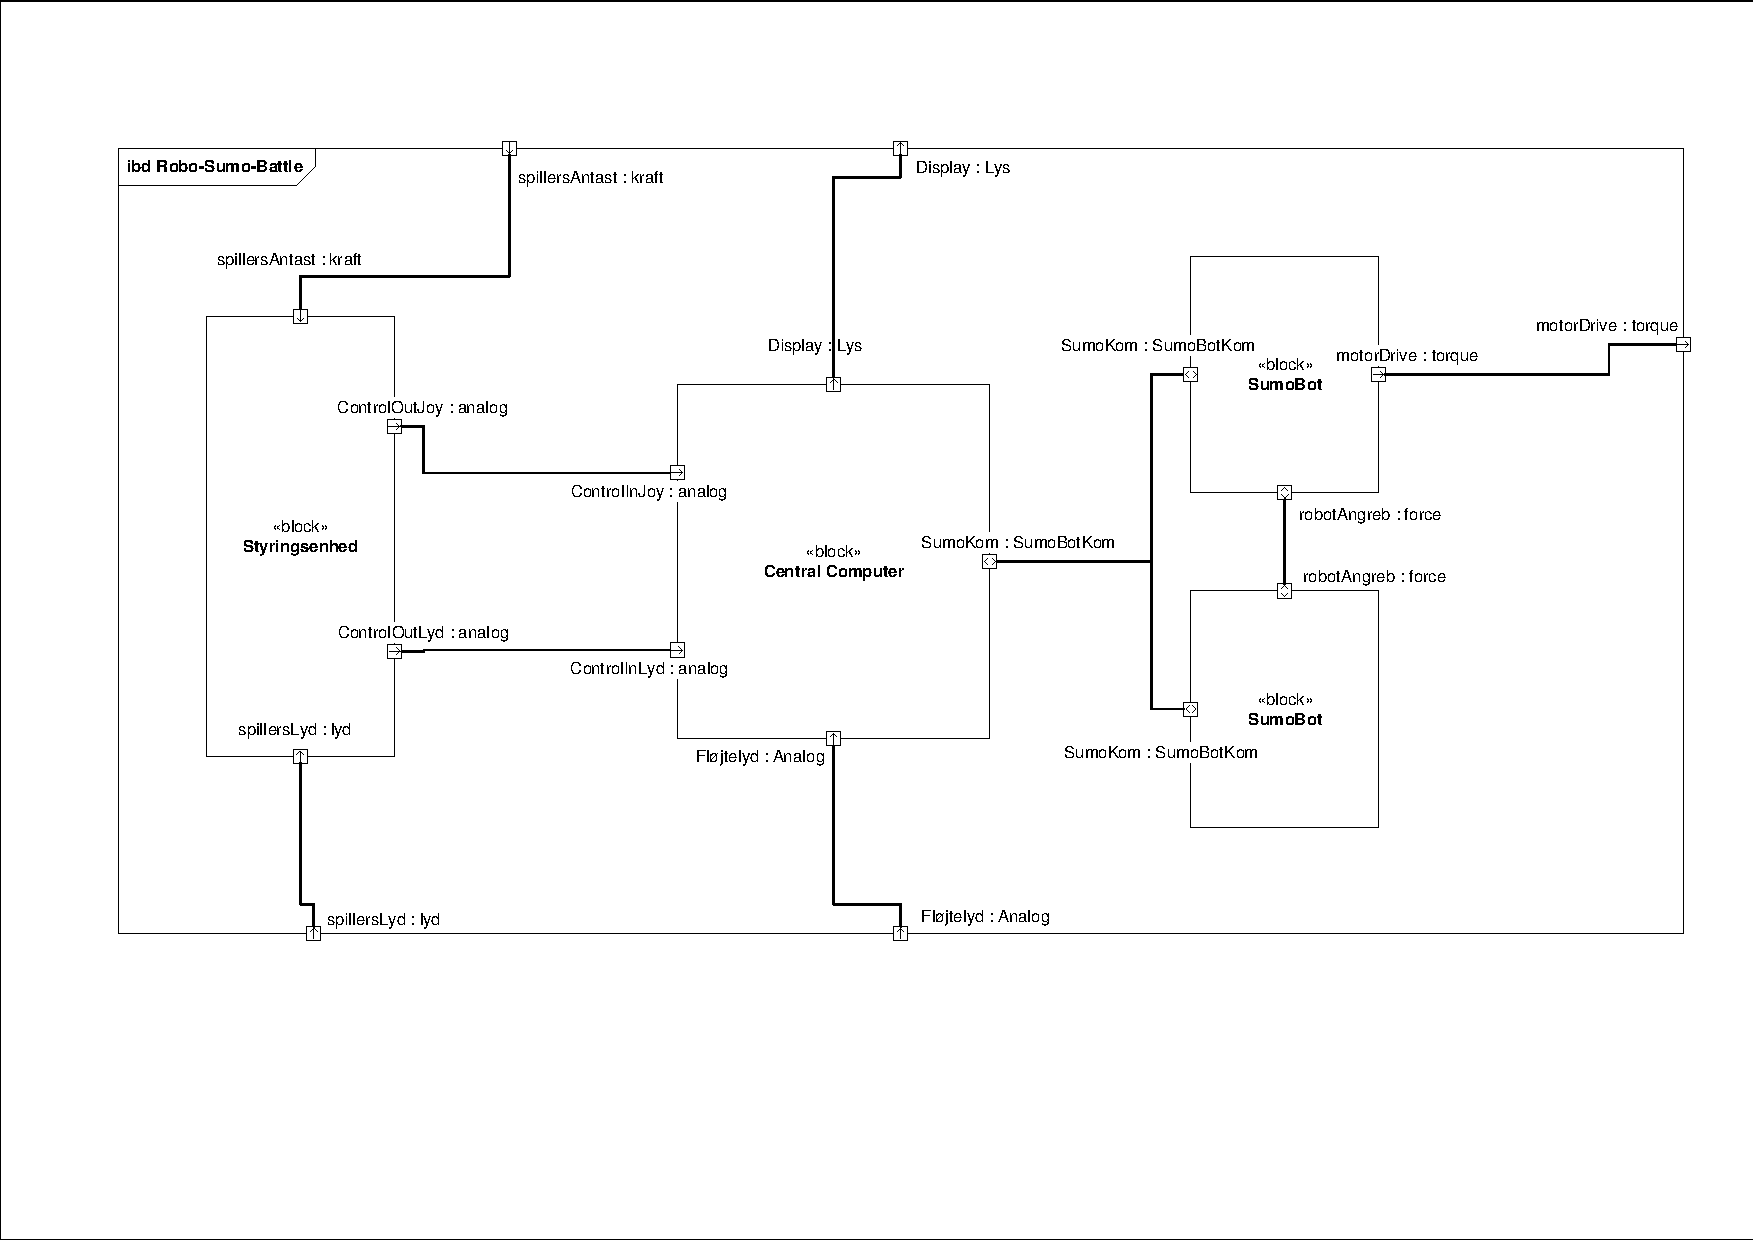
\includegraphics[page=1,width=1\linewidth]{figs/Diagrammer/IBD.pdf}
	\caption{System IBD}
	\label{fig:IBD_System}
\end{figure*}

\begin{figure*}
	\centering
   	\includegraphics[page=3,width=1\linewidth]{figs/Diagrammer/IBD.pdf}
	\caption{IBD for Central Computer, se \tabref{interface_table_CentralComputer} for interfacebeskrivelse}
	\label{fig:IBD_CentralComputer}
\end{figure*}
\begin{figure*}
	\centering
   	\includegraphics[page=2,width=1\linewidth]{figs/Diagrammer/IBD.pdf}
	\caption{IBD for Styringsenhed, se \tabref{interface_table_Styringsenhed} for interfacebeskrivelse}
	\label{fig:IBD_Styringsenhed}
\end{figure*}
\begin{figure*}
	\centering
   	\includegraphics[page=4,width=1\linewidth]{figs/Diagrammer/IBD.pdf}
	\caption{IBD for SumoBot, se \tabref{interface_table_SumoBot} for interfacebeskrivelse}
	\label{fig:IBD_SumoBot}
\end{figure*}

\subsection{Interface beskrivelser}
\noindent Der er udarbejdet en interface beskrivelse for de mere komplekse interfaces. For \figref{IBD_SumoBot} findes en dertilhørende interfacebeskrivelse i  \tabref{interface_table_SumoBot}.

\noindent For \figref{IBD_CentralComputer} findes en dertilhørende interfacebeskrivelse i \tabref{interface_table_CentralComputer}.
%%%%%%%%%%%%%%%%%
% 2020/10/24 - Adam
% Jeg har tilladt mig at "rydde" op i koden her, ved at tage udgangspunkt i UseCase.sty - Der er lavet et nyt environment \begin{SignalDescrption}{Navn}{label}
% Her i kan \signalbeskrivelse{navn}{type}{beskrivelse} skrives. - Se Grp6_tabels for mere info.
% Dette skulle gerne sikret et ensartet udtryk, samt et enkelt workflow. 
%%%%%%%%%%%%%%%%%
\begin{SignalDescription}{Central Computer}{CentralComputer}
    \signalbeskrivelse{in ctrlInJoy       }{Digital     }{Seriel forbindelse med defineret retning og hastighed}
    \signalbeskrivelse{in ctrlInLyd       }{Digital     }{Seriel forbindelse med defineret retning og hastighed}
    \signalbeskrivelse{out DisplayDataOut }{Digital Bus }{6 parallelforbindelser der overføre displayinformation}
    \signalbeskrivelse{out LCDOut         }{Light       }{Spilinformation til brugerne.}
    \signalbeskrivelse{inout robotKom     }{WIFI        }{Trådløs tovejskommunikation, til styring af SumoBot  og returnering af attacks }
\end{SignalDescription}

\begin{SignalDescription}{Styringsenhed}{Styringsenhed}
    \signalbeskrivelse{in ctrlInLyd    }{analog              }{\tbr Et lydsignal med frekvensindhold 100-10000 Hz}
    \signalbeskrivelse{in filterIn     }{analog              }{\tbr Lydsignal fra blokfløjte, muligvis overlejret med støj }
    \signalbeskrivelse{out joyStickOut }{                    }{\textbf{Bus med 5 signaler}:}
    \signalbeskrivelse{                }{1: analogX          }{spænding variende mellem 0 og VCC}
    \signalbeskrivelse{                }{2: analogY          }{spænding variende mellem 0 og VCC}
    \signalbeskrivelse{                }{3: digital          }{switch til at trykke på joystick controller}
    \signalbeskrivelse{                }{4:  VCC             }{5V}
    \signalbeskrivelse{                }{5: GND              }{0V}
    \signalbeskrivelse{out Mikrofon    }{analog              }{Udgangsimpedans 2,2k Ohm \tbr                               }
    \signalbeskrivelse{                }{                    }{Udgangsspænding 6,3 mV/Pa/1 kHz \tbr                        }
    \signalbeskrivelse{out ctrlOutJoy  }{analog              }{\tbr Samme som joyStickOut? Tilpasset i amplitude?          }
    \signalbeskrivelse{out ctrlOutLyd  }{\tbr analog/digital }{\tbr Interface til central computer                         }
\end{SignalDescription}
% \begin{table*}[]
%     \centering
%     \caption{Interfacebeskrivelse for Central Computer}
%     \label{tab:interface_table_CentralComputer}
%     \begin{tabular}{lp{5cm}p{7cm}}\toprule
%         Navn              & Type       & Beskrivelse\\                                                                                                                                 
%         in ctrlInJoy        & Digital    & Seriel forbindelse med defineret retning og hastighed\\
%         in ctrlInLyd        & Digital    & Seriel forbindelse med defineret retning og hastighed\\     
%         out DisplayDataOut  & Digital Bus     & 6 parallelforbindelser der overføre displayinformation\\
%         out LCDOut                & Light    & Spilinformation til brugerne.\\
%         inout robotKom       & WIFI              & Trådløs tovejskommunikation, til styring af SumoBot  og returnering af attacks\\
%         \bottomrule
%     \end{tabular}%
% \end{table*}

% \begin{table*}[]
%     \centering
%     \caption{Interfacebeskrivelse for Styringsenhed}
%     \label{tab:interface_table_Styringsenhed}
%     \begin{tabular}{lp{5cm}p{7cm}}\toprule
%         Navn              & Type       & Beskrivelse\\                                                                                                                                 
%         in ctrlInLyd      & analog     & \tbr Et lydsignal med frekvensindhold 100-10000 Hz\\
%         in filterIn       & analog     & \tbr Lydsignal fra blokfløjte, muligvis overlejret med støj\\                                                                                             
%         out joyStickOut   &            & Bus med 5 signaler:\\
%                           & 1: analogX & spænding variende mellem 0 og VCC\\                                                                                                        
%                           & 2: analogY & spænding variende mellem 0 og VCC\\                                                                                                            
%                           & 3: digital & switch til at trykke på joystick controller\\                                                                                                                
%                           & 4:  VCC    & 5V                                         \\                                                                                                      
%                           & 5: GND     & 0V                                         \\
%         out Mikrofon      & analog     & Udgangsimpedans 2,2k Ohm \tbr\\
%                           &            & Udgangsspænding 6,3 mV/Pa/1 kHz \tbr\\
%         out ctrlOutJoy & analog & \tbr Samme som joyStickOut? Tilpasset i amplitude?\\
%         out ctrlOutLyd & \tbr analog/digital & \tbr Interface til central computer\\                                                                                               
%         \\
%                 \bottomrule
%     \end{tabular}%
% \end{table*}

%% Analyse !
\chapter{Analyse}
\section{Central Computer Analyse}\label{sec:CC:analyse}

Analyseafsnittet vil for de to blokke i central computer yderligere udpensle krav til selve blokkene, såvel som forbindelserne imellem dem. Da denne del af systemet er software præget, vil der især blive lagt vægt på hvilke krav der stilles til de teknologier som skal understøtte specifikke funktionaliteter. 

Den centrale computers opgave er at fungere som det digitale bindeled mellem styringenhederne og SumoBots, således at den fra styringsenhederne modtager information som processeseres til retning og hastighed, som ultimativt kan blive videreformidlet til de to SumoBot's. Samtidig holder Central Computer styr på spillets status, dvs. antal liv, resterende spilletid mv. 

Central Computers funktionalitet er overordnet skitseret i \figref{Strukturering/Central Computer/SystemSekvensdiagram.png}

\fig{Strukturering/Central Computer/SystemSekvensdiagram.png}{0.55}{Central Computer System Sekvensdiagram}

%%% \begin{PartBlokDescription}{Styringsenhed: Mikrofon}{Styringsenhed:Mikrofon}  <- der kan du se hvordan jeg har sat label + titel op - hvis det giver mening :^)
% De eneste ændringer ift. BlokDescription er :      
%BlokDescription -> PartBlokDescription 
%Der er tilføjet [: Underblok] til både titel og label.
\subsection{Embedded Controller}
\label{sec:Embedded_Controller}

\fig{Analyse/CC/EmbeddedControllerIBDUdklip.png}{0.25}{Embedded Controller I/O}

\begin{PartBlokDescription}{Central Computer: Embedded Controller}{Central Computer Embedded Controller}
\Blokbeskrivelse{Embedded controller}{Bearbejder og videregiver data fra Styringsenhed til Sumobot, trådløst. sender løbende information  omkring  spilstatus (re-sterende liv, resterende spilletid mv.) til Display blokken}
\Portbeskrivelse{In Styringsprotokol}{SPI}{Digitalt samplet signal af detvalgte styringsinput (lyd eller  joystick)  fra  styringsen-hede}{
\item 
\item 
}
\Portbeskrivelse{Out displayData}{SPI}{Løbende information omkring spilstatus (re-sterende liv, resterende spilletid mv.)}{
\item 
\item 
}
\Portbeskrivelse{Inout SumoKom}{Wifi}{Tovejskommunikation  med  SumoBot’s  hvor  der  sendes information omkring retning og hastighed og modtage in-formation om et evt. angreb}{
\item 
\item 
}
\end{PartBlokDescription}

Embedded Controller ud- og indgange ses i  \figref{Analyse/CC/EmbeddedControllerIBDUdklip.png} 


Da afsnittet omfatter til den ene blok Embedded Controller, er dette afsnit yderligere inddelt ift. dens opgaver og interfaces. Kravene for de forskellige underafsnit skal ses som en samlet mængde krav til valg af Embedded Controller.

\subsubsection{Interface mod styringsenheden}
Interfacet til Styringsenheden modtager signalet Styringsprotokol som overføres jf. SPI-protokollen. Signalet er ikke proccesseret på dette tidspunkt og vil blot være en bitstrøm af samplede amplituder fra styringsenhedens lyd- eller controllerinput. Disse skal senere proccesseres til at blive en retning og en hastighed for en SumoBot. Controllerinputtet analyseres udelukkende ift. amplitude mens lydinputtet analyseres ift. amplituder indenfor specifikke frekvensspektre, som ultimativt vil give en retning og en hastighed. 

\textbf{Krav}
\begin{itemize}
\item Skal have indgange til minimum 2 SPI-forbindelser. En til hver Styringsenhed. 
\item SPI-indgangen skal kunne modtage data i en hastighed som stemmer overens med samplingsfrekvensen på >10kHz og bitopløsningen på 10 bit fastsat i afsnittet \ref{sec:Styringsenhed:analyse} \tbr. Det vil sige med denne sammenhæng: 
\[ F_s \cdot \text{bitopløsning} < \text{hastighed} \left[\si[per-mode=fraction]{\kilo\bit\per\second}\right] \]
\[ \text{hastighed} > 100.000 \left[\si[per-mode=fraction]{\bit\per\second}\right] \]
\end{itemize}

\subsubsection{Controllerbehandling}
\textbf{Lydbehandling}
Lyden som opfanges af mikrofonerne og sendes digitaliseret til Central Computer fra Styringsenhederne. Disse skal herefter proccesseres først vha. frekvensanalyse (diskret Fourier-transformation, herefter DFT). Den algoritme som danner baggrund for \gls{DFT} kræver meget processorkraft, som, særligt når behandlingen skal foretage så mange på hinanden følgende gange med kort tidsinterval. \gls{DFT} kommer ikke til at stå alene, da der efterfølgende vil være endnu en algoritme som omregner frekvensspektret til en retning og hastighed. 

\textbf{Krav}
\begin{itemize}
\item Processoren skal kunne arbejde med en høj clock-hastighed og gerne ved mange bits, således at det, samtidig med de resterende ting som foregår på processoren, er muligt at have to DFT som med kort tidsinterval foregår samtidig.  
\end{itemize}

\textbf{Joystikbehandling}
Behandlingen af inputtet fra joystikket er meget mere simpelt, da styringen igennem dette baserer sig på amplituden på signalet, som modtages fra styringsenheden digitaliseret og som blot vha. en simpel algorime omregnes til retning og hastighed. 

\subsubsection{Spilstyring}
Spilstyringen kan se som en state-machine som styrer resterende tid og liv for de to SumoBots. Spilstyringen skal programmeres i et sprog som egner sig hertil, hvortil der stilles krav om at det er overskueligt og gerne med et højt abstraktionsniveau, således at det er let at programmere og senere udbygge hvis der på et tidspunkt ønskes flere spiltilstande. Det skal igennem sproget være let at manipulere GPIO's, således at der spillets status let kan formidles til displayet. 

\subsubsection{Interface mod SumoBots (Trådløs kommunikation)}
Interfacet med SumoBots er en trådløs forbindelse som hostes af Central Computer og som SumoBots under opstart kobler sig på.
Informationen som formidles til SumoBots bliver efter en simpel protokol som sendes med korte tidsintervaller ($\approx$ 50ms). 

\textbf{Krav}
\begin{itemize}
\item Embedded Controller skal kunne lave et wifi-access point
\item Wifi-forbindelsen skal række min. 4 meter 
\item Wifi-forbindelsen skal være stabil
\end{itemize}

\subsection{Display}

\fig{Analyse/CC/DisplayIBDUdklip.png}{0.25}{Display I/O}

\begin{PartBlokDescription}{Central Computer: Display}{Central Computer Display}
\Blokbeskrivelse{Display}{Viser løbende information  omkring  spilstatus  (resterende liv, resterende spilletid mv.) til spillerne}
\Portbeskrivelse{Out Display}{Lys}{Displayets løbende information til spillerne omkring spilstatus (resterende liv, resterende spilletid mv.)}{
\item 
\item 
}
\Portbeskrivelse{In displayData}{SPI}{Løbende   information   om-kring spilstatus (re-sterendeliv, resterende spilletid mv.)}{
\item 
\item 
}
\end{PartBlokDescription}

Displayet fungere som kommunikationsportalen mellem spillet og dets spillere. Igennem et spil vil der løbe en informationsstrøm fra systemet til brugerne, der dieregere dem gennem spillets forløb. I det ligger der Information vedrørende resterende liv af spillernes respektive SumoBots, resterende spilletid, nedtælling til spillestart mv. Med andre ord sørger display blokken for at udføre kravet "Systemet \textbf{SKAL} kunne infomere spilleren om spillets status (nedtælling til start, SumoBotsrestenende liv, resterende spilletid)" som findes under \ref{Kravliste}. Der er på baggrund af dette krav blevet listet en række funktionelle krav:

\textbf{Krav}\label{Display_funktionelle_krav}
\begin{itemize}
\item Størelse på min 4x20 felter.
\item Skal benytte I2C kommunikation.
\item Fysisk størrelse på min 50*20mm, max 300*120mm

\end{itemize}
\clearpage
{
\def\dirfigs{figs/Analyse/Styringsenhed/}
\section{Styringsenhed}\label{sec:Styringsenhed:analyse}
\subsection{Lydgiver}\label{subsubsec:Styringsenhed:analyse:Lydgiver}
Der er blevet foretaget en analyse af forskellige lydinputs til systemet. Analysen består af en måleserie, hvor man med forskellige lydinputs skal afgøre, om det er muligt at isolere 4 frekvensbånd indenfor en rimelig frekvensopløsning og derved generere styrings-outputs ud fra disse. Målingerne er foretaget ved følgende procedure:
\begin{itemize}
    \item Indspilning af 4 forskellige toner af 3 omgange med samplefrekvens på 10 kHz.
    \item Mikrofonen benyttet er den indbyggede i en Lenovo T440p, lydkilde ca. 0,5 meter fra mikrofonen, samt et åbnet vindue ned til en trafikeret vej til at agere baggrundsstøj.
    \item Lydfilerne eksporteres som .wav fil og indlæses i Matlab.
    \item Lydfilerne processeres i Matlab til at et frekvensspektrum der vurderes muligt til at diskriminere lydinputtet til 4 styringsoutputs er opnået. 
    \item Det endelige resultat afspejler valget af lydinput samt specifikationerne for styringsenheden.
\end{itemize}

\subsubsection{Mandestemme}
\fig{ToneAnalyse/Voice_FFT_Close_N_512}{.7}{Mandestemme, 4 toners frekvensspektrum}

I Figur \ref{fig:ToneAnalyse/Voice_FFT_Close_N_512} ses et frekvensspektrum af en mandestemme, der for så vidt muligt har forsøgt at generere 4 forskellige toner. Her er påført hann-vindue for at minimere sidesløjfer og foretaget en 256 punkters FFT.

Dette giver anledning til følgende vurdering:
\begin{itemize}
    \item Der sættes alt for høje krav til aktøren om at ramme bestemte toner, hvis der ikke indføres en talegenkendelsesstandard. Alene ud fra denne praktiske overvejelse forkastes stemmer som inputs. 
\end{itemize}
\subsubsection{Blokfløjte}\label{subsubsec:Styringsenhed:analyse:Mundharmonika}

\fig{ToneAnalyse/Recorder_FFT_N_128}{.7}{Blokfløjte, 4 toners frekvensspektrum, 64 bins FFT}
\fig{ToneAnalyse/Recorder_FFT_N_512}{.7}{Blokfløjte, 4 toners frekvensspektrum, 256 bins FFT}

I \figref{ToneAnalyse/Recorder_FFT_N_128} og \figref{ToneAnalyse/Recorder_FFT_N_512} ses frekvensspektrummet for en aktør som har spillet 4 forskellige toner (2 fingre på, 4 fingre på, 6 fingre på og 8 fingre på for at udnytte mest muligt af frekvensområdet). Her er ganget et hann-vindue på signalet for at minimere sidesløjfer og der er hhv. foretaget en 64 og 256 punkters FFT. Dette giver anledning til følgende konstateringer og vurdering:
\begin{itemize}
    \item Signalfrekvensområde ca. 550 Hz - 1150 Hz.
    \item Frekvensområde for hvert tone ca. 100 Hz.
    \item Her er 40 dB niveauforskel fra tone 4 til tone 3 (ca. 60 Hz) med frekvensopløsning $F_s/2/256 = 19,56 Hz$.
    \item SNR på ca. 40 dB (fra top af noise floor til top af peaks)
    \item Det ses, at tonerne rammes klart. Her har der dog for aktørens vedkommende været god tid til at ramme tonerne. I en realtids-applikation vurderes det for omfangsrigt for aktørens motorik at ramme tonerne.
    \item Blokfløjten er amplitudeafhængig på en meget negativ måde. Man skal være meget påpasselig for ikke blot at ende i oversvingningerne.
    \item Med tilført hann-vindue og 256 punkters FFT vurderes det muligt at diskriminere signalindholdet til 4 outputs, men på baggrund af de praktiske overvejelser, overvejes yderligere lydinputs. 
\end{itemize}

\subsubsection{Mundharmonika}
Samme procedure følges for en mundharmonika som lydinput. Som en modifikation for at imødekomme det praktiske problem i at ramme tonerne, er der ved hjælp af elastikker dannet 4 "firkanter" som man kan puste i. 

\fig{ToneAnalyse/FFT_Close_N_128}{.7}{Mundharmonika, 4 toners frekvensspektrum, 64 bins FFT}

\fig{ToneAnalyse/FFT_Close_N_256}{.7}{Mundharmonika, 4 toners frekvensspektrum, 128 bins FFT}

\fig{ToneAnalyse/FFT_Close_N_512}{.7}{Mundharmonika, 4 toners frekvensspektrum, 256 bins FFT}

I \figref{ToneAnalyse/FFT_Close_N_128}, \figref{ToneAnalyse/FFT_Close_N_256} og \figref{ToneAnalyse/FFT_Close_N_512} ses lydsignalet fra de 4 toner genereret af mundharmonikaen. Der er ganget et hann-vindue på for at minimere sidesløjfer.
%Der undersøges i \figref{ToneAnalyse/NoHannFFT_Close_N_512}, om hann-vinduet er nødvendigt. 

%\fig{ToneAnalyse/NoHannFFT_Close_N_512}{.7}{Mundharmonika, 4 toners frekvensspektrum, 256 bins FFT - ubehandlet}

%Ud fra \figref{ToneAnalyse/NoHannFFT_Close_N_512} vurderes det nødvendigt at tilføje et hann-vindue til indgangssignalet. 

Dette giver anledning til konstateringen og vurderingen:
\begin{itemize}
    \item Signalfrekvensområde ca. 200-1250 Hz.
    \item Frekvensområde for hver tone mindst ca. 150 Hz (tone 1) og højest ca. 250 Hz (tone 3).
    \item 40 dB niveauforskel fra den ene tone til den anden (mindst overgang fra tone 2 til tone 3, ca. 60 Hz. Og højest overgang fra tone 3 til tone 4, ca. 100 Hz) med frekvensopløsning $F_s/2/256 = 19,56 Hz$.
    \item SNR på ca. 40 dB (fra top af noise floor til top af peaks)
    \item Det ses, at tone 3 og tone 4 i \figref{ToneAnalyse/FFT_Close_N_512} rammes nemmere end de andre. Dog observeres også, at amplituden kun hæver niveau og ikke frekvens, hvilket var en faldgrube ved blokfløjten. 
    \item Med "støtten" i form af elastikker på mundharmonikaen er det nemt at ramme tonerne rigtigt.
\end{itemize}

\subsubsection{Endelig beslutning af lydgiver}
Selvom blokfløjtens frekvensspektrum i \figref{ToneAnalyse/Recorder_FFT_N_512} ser lovende ud, forkastes denne mulighed udelukkende af de ovenstående drøftede praktiske årsager. Hertil vurderes mundharmonikaen til at være et tilstrækkeligt alternativ. Her er større frekvensbånd for hver tone og større frekvensområde til overgangen mellem frekvensbåndene, hvilket gør det lettere at skelne tonerne fra hinanden og derved arbejde med for at generere styringsoutputs. 

\subsubsection{Krav til styringsenhed ud fra lydgiver}
Hermed kan følgende krav for de andre enheder i styringsenheden fastsættes:
\begin{itemize}
    \item Signalfrekvensområde: 200-1250 Hz.
    \item Skal kunne isolere 4 toner med en overgang på højest 100 Hz i signalfrekvensområdet.
    \item I sammenhæng med kravet stillet i \ref{sumobotkrav} skal ovenstående udføres på under et sekund (inklusiv eventuelle forsinkelser i de andre subsystemer).
    \item Signal-støj-forhold på 40 dB gennemgående i signalkæden.
\end{itemize}

\subsection{Mikrofon}
\fig{styringsenhed_mikrofon}{0.4}{Udsnit af mikrofonblokken}
\begin{PartBlokDescription}{Styringsenhed: Mikrofon}{Styringsenhed:Mikrofon}
\Blokbeskrivelse{Mikrofon}{Konvertering fra akustisk til elektrisk signal}
\Portbeskrivelse{Mikrofon}{Analog}{}{
\item Udgangsimpedans: 2.2\kohm 
\item Sensitivitet: \SI{8(2)}{\milli\volt\per\pascal}
\item SNR: 40dBV
}
\Portbeskrivelse{SpillersLyd}{Akustisk}{}{
\item Dynamisk område: 70dB SPL
\item Signalfrekvensområde: 250 til 1.55 kHz
}
\end{PartBlokDescription}

\subsubsection{SNR og dynamisk område}
Ud fra kravene i Afsnit \ref{subsubsec:Styringsenhed:analyse:Lydgiver} vurderes, at en standard elektretmikrofon \tbr (link til mikrofon), som allerede var til rådighed, vil kunne opfylde kravet.
Med et signal-støj-forhold opgivet til 58 dB vil dette ende i et akustisk dynamisk område på ca. 70dB\cite{Lewis2012}, hvilket vurderes tilstrækkeligt til at opfange inputs fra mundharmonikaen. 

Hvis baggrundsstøjen er i et større omfang end hidtil regnet med i afsnit \ref{subsubsec:Styringsenhed:analyse:Lydgiver}, så baggrundsstøjen ikke kan differentieres fra det reelle input, vil der i implementeringen skulle laves akustisk regulering.

\subsubsection{Sensitivitet}
Sensitiviten for den valgte mikrofon er opgivet til \SI{8(2)}{\milli\volt\per\pascal}, hvorfor der fra denne specifikation interfaces videre til en bestemmelse af forstærkerkredsløbets gain.

\subsection{Analog signalbehandling}
\fig{styringsenhed_analogsignalbehandling}{0.4}{Udsnit af blokken til analog signalbehandling}
\begin{PartBlokDescription}{Styringsenhed: Analog signalbehandling}{Styringsenhed:Analogsignalbehandling}
\Blokbeskrivelse{Analog signalbehandling}{Forstærker mikrofon inputtet i en grad at ADC kan konvertere de forskellige værdier. \newline Gain: 250gg}
\Portbeskrivelse{Lydsignal}{Analog}{Ufiltreret og forstærket signal indeholdende lydinformation.}{
\item Indgangsimpedans: Høj
}
\Portbeskrivelse{Behandlet lydsignal}{Analog}{Filtreret og forstærket signal indeholdende lydinformation.}{
\item Signalfrekvensområde: \SIrange{200}{1250}{\Hz}
\item Udgangsimpedans: Lav
}
\end{PartBlokDescription}


Denne blok skal filtrere frekvenser udenfor pasbåndet fra samt forstærke signalet fra mikrofonen op, så det kan registreres af en ADC.

Det er nødvendigt at have et filter der uden problemer kan lukke frekvenser i området liggende fra \SIrange{250}{1500}{Hz} igennem, uden at det opstår bemærkelsesværdi forvrængning eller faseproblemer, derudover bør uønskede frekvenser bortfiltreres i en grad af de ikke opfanges af ADC'en.

Med et pasbånd beliggende i området \SIrange{250}{1550}{Hz} og en dertilhørende forstærkning på \ca{300}, vil et passende frekevensrespons være et båndpasfilter der kan beskrives : 
\begin{equation}
    T(s) = T_{\textrm{HP}} \cdot T_{\textrm{LP}} \cdot T_{\textrm{Gain}} 
\end{equation}
hvor følgende gør sig gældende for de forskellige led
\begin{equation}
    \begin{split}
        T_{\textrm{HP1}} &= \fdb = \SI{250}{Hz} \quad \SI{20}{\dB\per dec} \\
        T_{\textrm{LP1}} &= \fdb = \SI{1550}{Hz} \quad  \SI{40}{\dB\per dec} \\
        T_{\textrm{Gain}} &= \textrm{Gain} \approx  300
    \end{split}
\end{equation}


\subsection{Signalkonditionering}
\fig{styringsenhed_signalkonditionering}{0.4}{Udsnit af blokken til signalkonditionering}

\begin{PartBlokDescription}{Styringsenhed: Signal konditionering}{Styringsenhed:Signalkonditionering}
\Blokbeskrivelse{Signal\newline kondition-ering}{Buffer stage der skal sikre maksimal spændings-overførsel.}
\Portbeskrivelse{Behandlet lydsignal}{Analog}{}{
\item Indgangsimpedans: 10x udgangsimpedans for Analog Signalbehandling blokken.
}
\end{PartBlokDescription}

\subsection{ADC}
\fig{styringsenhed_adc}{0.4}{Udsnit af ADC-blokken}

\begin{PartBlokDescription}{Styringsenhed: ADC}{Styringsenhed:ADC}
\Blokbeskrivelse{ADC}{Analog til digital konvertering.}
\Portbeskrivelse{ADCinLyd}{Analog}{}{
\item Fuld skala input spændingsområde: \SIrange{0}{5}{\volt}
\item Indgangsimpedans: høj
\item Sample rate: 10 kHz.
\item Bitopløsning: 8 bit
\item SNR: 40 dB
}
\Portbeskrivelse{adcOutLyd}{Digital}{Array med værdier fra ADC med tilstrækkelig plads til at foretage en FFT ud fra Digital Signal Processerings-blokkens bestemte specifikationer}{
\item Type: uint8
}
\end{PartBlokDescription}

\subsubsection{ADCinLyd}
Fuld skala input range på ADC'ens indgang skal stemme overens med inputsignalets spændingsområde for at udnytte hele inputsignalet og derved sikre maksimal opløsning. 
Derfor fastsættes at fuld-skala input range = 5V.

Når signal-støj-forhold på 40 dB er vurderet som tilstrækkeligt, kan denne værdi bruges som udgangspunkt til et mindstekrav for bitopløsningen,\cite{KesterMT-001Care}, som ADC'en skal outputte med:
\[ 40 = 6.02 \cdot n+1.76 \]
\[ n = 6.37 \to n = 8 \]

Der skal altså anvendes en ADC med en effektiv bitopløsning på mindst 6.37. Der vælges derfor at anvende en ADC med 8 bit opløsning. 

\subsubsection{adcOutLyd}
Denne specifikation er givet ud fra bitopløsningen på ADC'en samt specifikationerne for Digital Signal Processing. Se yderligere overvejelser herfor i afsnit \ref{Digital:Signal:Processing}. 

\subsection{Digital Signal Processing}\label{Digital:Signal:Processing}
\fig{styringsenhed_dsp}{0.4}{Udsnit af ADC-blokken}
For at skabe et styringssignal der kan sendes videre i systemet, er nødvendigt at processere den \emph{samplede} data med henblik på at identificere de 4 toner der er angivet i \nameref{subsec:Styringsenhed:analyse:Mundharmonika}. %\ref

Der er  flere metoder der kan nå det samme resultat, hvor to af disse er vist i \tabref{Styringsenhed:analyse:DSPMetoder} hvor det ses at de to metoder givet vis kan det samme, de implementeres blot på to forskellige måder--- det gør dem dog ikke ens.

\begin{table}[!h]
	\small
	\centering
	\caption{DSP isoleringsmetoder}
	\label{tab:Styringsenhed:analyse:DSPMetoder}
	\begin{tabular}{lll}
		                                           & \multicolumn{1}{c}{FFT} & \multicolumn{1}{c}{4 $\times$ Båndpasfilter} \\\midrule
		Kan implementeres på embedded controller   & \checkmark              & \checkmark                              \\
		Kan implementeres ud fra analyseresultater & \checkmark              & \checkmark                              \\
		Total udnyttelse af data                   &                         & \checkmark                              \\
		Mulighed for læseligt output                      & \checkmark              & \checkmark                              \\
		Kendskab fra AU Kurser                     & \checkmark              & \checkmark                              \\
		Litteratur                                 & \checkmark              & \checkmark                              \\\bottomrule
	\end{tabular}
\end{table}
\subsubsection{FFT metode}
FFT metoden vil med 512 input samples, som vist i \figref{ToneAnalyse/FFT_Close_N_512}, producere 256 \emph{FFT-bins}\cite{DigitalSignalProcessing} i et frekvensdomæne, hvor hver bin er med en opløsning der beskrives $\sfrac{\textrm{Samplerate}}{\textrm{Antal FFT bins}}$, dog skal kun 4 enkelte frekvensområder isoleres --- hvor der udfra \figref{ToneAnalyse/FFT_Close_N_512} ses at 2 til 3 bins pr. isoleret tone vil være tilstrækkeligt i tilfældet $N=512$, vil dette medføre et samlet \emph{spild} der kan beskrives \[\textrm{Binspild} = \textrm{Antal FFT bins} - (\textrm{Isolerede toner} \times  \textrm{Antal tonebins}).\]
Dette spild kan vise sig at være problematisk i form at tidsudregninger, og dette bør derfor i designfasen optimeres til et punkt hvor dataspild er på et minimum. 

Selve FFT-metoden vil kræve $X$ antal udregninger inklusiv spildet, hvor $X$ kan beskrives 
\(\tfrac{\textrm{Antal Samples}}{2} \times  \log_2 (\textrm{Antal Samples})\), dette bør dog ikke vise sig som værende et problem da platformen hvorpå metoden skal afvikles, har tilstrækkelig regnekraft til at kunne udføre disse operationer uden problemer\cite{Bronshtein2015,PSoC5LPDatasheet}.

%%%% 
\subsubsection{$4 \times$ digital båndpasfilter}

Det vil også være muligt at isolerere de fire toner ved at isolere dem med en række filtre. Her ville et antal båndpas filtre, hvor der i designfasen udarbejdes filtertyper der kan isolere de fire interessetoner.
Dette er dog ikke en metode er vil gåes videre med, da arbejdet med FFT metoden vægtes højere, da lærings/udviklings-processen i denne er noget der ønskes udforsket fra gruppens side.

Dog forkastets båndpasmetoden ikke, da denne bør kunne implementeres i stedet for FFT-metoden uden de store armbevægelser hvis sidstnænvte metode ikke viser sig tilstrækkelig eller volder problemer der er for tidskrævende at rette op.

}























\clearpage
\section{Sumobot Analyse}\label{sec:Sumobot:analyse}

I dette analyseafsnit vil der indledningsvis blive lavet analyse for de essentielle elementer for SumoBot, der vil lægge grundlag for kravene af de enkelte delblokke. Foruden analysen, vil ansvaret for de enkelte delblokke blive fremstillet. Ydermere beskrivelsen af blokkene, vil forbindelserne mellem dem såvel blive udpenslet. Afsluttende vil der blive stillet en række krav for selve blokkene, der bliver grundlag for valg af komponenter senere i rapporten.


\subsection{Sumobot Del Analyse}\label{subsubsec:SumoBot:Analyse}

\subsubsection{Nødvendig trækkræft}
Et kristisk område at lægge en del fokus, er elementet, der flytter objektet, SumoBot, hen over spillepladen. Som nævnt i kravspecifikationen, afsnit \ref{sumobotkrav}, vil SumoBot have en maksvægt på 2,5 kg og begrænsende dimensioner på maks 20cmx20cmx20cm. Der ligger altså et analyseområde i at bestemme et momentkrav der skal til at flytte objektet, der samtidig overholder størrelseskravet.

Der er blevet foretaget en analyse af det nødvendige moment motorene skal generere på hjulakslerne før bilen ville kunne flytte sig over banen.
For at dette kunne beregnes er følgende antagelser blevet anvendt:
 \begin{itemize}
   \item Tab i aksel og lejer samt i en eventuelt anvendt gearing osv. er en antaget at være en konstant på 0,9. Med andre ord antages der at effektoverførelsen mindskes med 10\%.
   \item Gnidningsoverfladerne mellem hjul og underlag, antages at være mellem gummi og beton. 
   \item Vægtfordelingen på SumoBotten er ligeligt fordelt. Denne vægt antages desuden af være fordelt på 2 hjul, hvilket betyder at eventuelle støttehjul ses bort fra da de kun anses for at holde balancen og ikke decideret bærer nogen vægt.
\end{itemize}

\subsubsection{Moment beregning}
Ved udregning af det nødvendige moment, kan de forskellige faktorer der spiller ind, simplificeret, opdeles i 3 elementer, der summeret angiver det nødvendige moment der kræves, til at flytte det specifikke objekt i de specifikke omgivelser.
De 3 elementer er henholdsvis:

\begin{itemize}
    \item Rullemodstanden
    \item Hældningsmodstanden
    \item Accelerationskraften
\end{itemize}

Der indskrives de nødvendige værdier fra overordnede krav til systemet samt de fysiske love og antagelser:

\begin{flalign*}
  \text{RulleModstand for beton og gummi} && Crr &= 0.015 &\\
  \text{Vægt af SumoBot} && GVW &= 2.5 KG &\\
  \text{Hældning af Banen} && Angle &= \deg{(0)} &\\
  \text{Ønskede Acceleration} && a &= 1 \frac{\mathrm m}{\mathrm s^2} &\\
  \text{Tyngdeacceleration} && g &= 9.807 \frac{\mathrm m}{\mathrm s^2} &\\
  \text{Tab i gear etc.} && R_f &= 0.9  &\\
  \text{Radius af hjulene} && R_w &= 0.04 m
\end{flalign*}

Dette giver anledning til følgende udregninger:

\begin{flalign*}
  \text{RulleModstand af SumoBot} && RR &= Crr \cdot GVW && RR = 0.038 kg &\\
  \text{Hældningsmodstanden} && GR &= GVW \cdot \sin{(Angle)} && GR = 0 kg &\\ 
  \text{Samlet masse af SumoBot} && m &= \frac{\mathrm GVW}{\mathrm g} && m = 0.255 \frac{\mathrm kg \cdot s^2}{\mathrm m}  &\\
  \text{Accelerationskraften} && FA &= m \cdot a && FA = 0.255 kg &\\
  \text{Minimum trækkraft nødvendig} && TTE &= RR + GR + FA && TTE = 0.292 kg &\\
  \text{Minimumskrav med 1 hjul} && T &= R_f \cdot TTE \cdot R_w && T = 1.053 kg \cdot cm &\\
  \text{Minimumskrav ved 2 hjul} && T_m &= \frac{\mathrm T}{\mathrm 2} && T_m = 0.526 kg\cdot cm&\\
\end{flalign*}

Det vil sige, at ifølge udregningen, da vil det kræve et minimumsmomentkrav på "0.526 kg-cm" pr. motor, at få Sumobot med fuld vægtbelastning til at accelerer med \SI{1}{\meter\per\second\squared}. 

 \figref{Strukturering/SumoBot/systemSekvensDiagram_SumoBot.png}
Ud fra den overordnede analyse "delafsnit X" af systemet udearbejdes der nogle krav til de enkelte delblokke samt beskriver deres
funktionalitet.

\fig{Strukturering/SumoBot/systemSekvensDiagram_SumoBot.png}{0.8}{SumoBot System Sekvensdiagram}


\subsection{Attack Sensor}
\fig{Analyse/SumoBot/ibd_sumobot_attacksensor.png}{0.60}{Attack Sensor IBD}

\begin{PartBlokDescription}{Attack Sensor}{}
\Blokbeskrivelse{Attack Sensor}{Registrere påkørsel mellem SumoBots. Kollisionsstatus sendes til Microcontroller.}
\Portbeskrivelse{pakoersel}{Force}{Fysisk påvirkning fra omverdenen}{
\item  \SIrange{0}{3.3}{\volt}  signal
}

\Portbeskrivelse{pakoertSignal}{Digital}{Logisk I/O signal}{
\item Spændingsområde: \SIrange{0}{3.3}{\volt}
}
\BlokSpacer{0cm}
\end{PartBlokDescription}

Attack Sensor er den del af SumoBotten der registrerer at den er blevet påkørt af en anden SumoBot.
2-3 Attack Sensorer monteres på bagsiden af hver SumoBot og registrere kollision.
På baggrund af funktionaliteten af sensoren, lægges der stor fokus på robustheden i valget af sensor. 

\textbf{Krav}
\begin{itemize}
\item Skal kunne registrere vandret tryk fra sumobot.
\item Skal kunne håndtere 5V med mellem 0 og 20 mA.
\item Skal kunne holde til minimum 10000 tryk.
\end{itemize}


\subsection{PSU}
\fig{Analyse/SumoBot/ibd_sumobot_psu.png}{0.40}{PSU IBD}

\begin{PartBlokDescription}{PSU}{}
\Blokbeskrivelse{PSU}{Forsyner de enkelte blokke med korrekt spændingsniveau. Kilden kommer fra batteri.}
\Portbeskrivelse{MCPower}{DC}{Forsyning til Microcontroller}{
\item Spændingsforsyning 5V
}
\Portbeskrivelse{PowerBat}{DC}{Batteri forsyning}{
\item Spændingsniveau: 9V
}
\BlokSpacer{0cm}
\end{PartBlokDescription}

Delblokken PSU er strømforsyningen, der skal levere et stabilt 5V DC signal til de interne komponenter. Det er vigtigt at den kan levere et stabilt signal så komponenterne ikke slukker eller genstarter pga. for høj eller lav spænding.
Derefter skal den også kunne videresende Batteri forsyningen til Motorstyringen.
Nedenstående krav er specificeret ved 25 grader celsius. 
\\
\textbf{Krav}
\begin{itemize}
\item Skal kunne levere en stabil 5V DC forsyning  med maks afvigelse på  4.80 < 5.00 < 5.20 V ved 25 grader.
\item Skal kunne lervare minimum 500 mA.
\item Skal kunne køre stabilt med et 7 til 12V DC input.
\item Skal kunne videresende Batteri forsyningen.
\item Må ikke fylde mere end 4x4x4 cm
\item Må maks have en output noice voltage på 120 mikroVolt
\end{itemize}

\subsection{Microcontroller}

\fig{Analyse/SumoBot/ibd_sumobot_microcontroller.png}{0.45}{Microcontroller IBD}

\begin{PartBlokDescription}{Microcontroller]}{}
\Blokbeskrivelse{Microcontroller}{Styrer motorstyringen ud fra indput fra Central Computer. Ligeledes har MicroControlleren forbindelse med Attack Sensoren og sender dataen videre til Central Computeren.}
\Portbeskrivelse{robotKom}{ SumoBotKom}{WIFI kommunikation fra og til Central Computeren}{
\item trådløs kommunikation mellem Central Computeren og MicroControlleren
}
\Portbeskrivelse{pakoerselRegistrering}{Digital}{Logisk I/O signal fra Attack Sensor}{
\item Spændingsområde: \SIrange{0}{3.3}{\volt}
}
\Portbeskrivelse{motorCmdOutLeft}{Signal}{Signal til motorstyring om venstre motor bestående af 2 logiske signaler og 1 PWM signal}{
\item logisk signal [2] med Spændingsområde: \SIrange{0}{3.3}{\volt}
\item PWM signal med Spændingsområde: \SIrange{0}{3.3}{\volt}
}
\Portbeskrivelse{motorCmdOutRight}{Signal}{Signal til motorstyring om højre motor bestående af 2 logiske signaler og 1 PWM signal}{
\item logisk signal [2] med Spændingsområde: \SIrange{0}{3.3}{\volt}
\item PWM signal med Spændingsområde: \SIrange{0}{3.3}{\volt}
}
\BlokSpacer{0.2cm}
\end{PartBlokDescription}

Microkontrolleren er den del af SumoBotten der styrer motorstyringen ud fra indput fra Central Computeren over WIFI. Det er også denne der er forbundet med Attack Sensoren. Af den grund skal mircocontrolleren være hurtig nok til at bearbejde dataen og modtage/sende det videre, samt styre motorstyring og registrere attack sensoren.
\\
\textbf{Krav}
\begin{itemize}
\item Skal kunne kommunikere  over WIFI.
\item Skal have minimum 10 In/Out ben.
\item Skal kunne køre 5V DC.
\item Skal kunne levere mellem 3.3V og 5V DC på output benene.
\item Må Maks være 12x4x4 cm.
\end{itemize}


\subsection{Batteri}
\fig{Analyse/SumoBot/ibd_sumobot_batteri.png}{0.40}{Batteri IBD}

\begin{PartBlokDescription}{Batteri]}{}
\Blokbeskrivelse{Batteri}{Forsyner PSU samt motorerne gennem motorstyringen.}
\Portbeskrivelse{chargePowerIn}{DC}{Til batteri fra oplader}{
\item Spændingsniveau: 9V
}
\Portbeskrivelse{PowerBat}{DC}{Fra batteri}{
\item Spændingsniveau: 9V
}
\BlokSpacer{0.4cm}
\end{PartBlokDescription}

I og med at Sumobot er trådløs, er det essentielt at have et batteri monteret, hvilket er det blokken \textit{batteri} står for. Men da robotten har en fysisk begrænsning, må batteriet ikke være for stort. Derudover skal batteriet levere et hvis spændingsniveau, som kan forsyne de forskellige delmoduler.
\\
\textbf{Krav}
\begin{itemize}
\item Må maks være 10x10x5 cm. \tbr
\item Skal kunne levere 2.5 Ampere.
\item skal have minimum 1000 mAh. \tbr
\item 9 V spænding\tbr
\end{itemize}


\subsection{Motor}
\fig{Analyse/SumoBot/ibd_sumobot_motor.png}{0.48}{Motor IBD}

\begin{PartBlokDescription}{Motor]}{}
\Blokbeskrivelse{Motor}{Skaber fremdrift/bevægelse til Sumobot. Bliver kontrolleret gennem motorstyringen.}
\Portbeskrivelse{motorCtrlIn[2]}{PWM}{PWM fra motorstyring til motor}{
\item PWM signal med Spændingsområde: \SIrange{0}{9}{\volt}
}
\Portbeskrivelse{motorTorqueOut}{torque}{Energi fra motor til hjul}{
\item Moment/energi fra motor til hjul \tbr
}
\BlokSpacer{0cm}
\end{PartBlokDescription}

Blokken \textit{motor} repræsenterer selve motoren. Dens opgave er at flytte SumoBot rundt på spillepladen.
I valg af motor sætter de fysiske dementioner (20x20x20) af SumoBot atter en begrænsning. Et andet aspekt der er værd at tage i betragtning er momentet i valget af motor.
Et andet aspekt i valg af motor, er at hver bil består af 2 motorer. Der skal altså i alt bruges 4 styk til projektet. \tbr
\\

\textbf{Krav}
\begin{itemize}
\item Skal have et moment på minimum 0.526 kg-cm.
\item Skal være en DC motor.
\item Må maksimalt være være 8x4x4 cm med akse.
\end{itemize}

\subsection{Motorstyring}
\fig{Analyse/SumoBot/ibd_sumobot_motorstyring.png}{0.36}{Attack Sensor IBD}

\begin{PartBlokDescription}{Motorstyring}{}
\Blokbeskrivelse{Motorstyring}{Styrer retning og hastighed af de 2 motorer ud fra kommandoer givet af Microcontrolleren.}
\Portbeskrivelse{motorCommandInRight}{Signal}{Signal til motorstyring om venstre motor bestående af 2 logiske signaler og 1 PWM signal}{
\item logisk signal [2] med Spændingsområde: \SIrange{0}{3.3}{\volt}
\item PWM signal med Spændingsområde: \SIrange{0}{3.3}{\volt}
}
\Portbeskrivelse{motorCommandInLeft}{Signal}{Signal til motorstyring om højre motor bestående af 2 logiske signaler og 1 PWM signal}{
\item logisk signal [2] med Spændingsområde: \SIrange{0}{3.3}{\volt}
\item PWM signal med Spændingsområde: \SIrange{0}{3.3}{\volt}
}
\Portbeskrivelse{motorCtrlOut[2]}{PWM}{PWM signal til motor}{
\item PWM signal med Spændingsområde: \SIrange{0}{9}{\volt} 
}

\end{PartBlokDescription}

Motorstyringen tager sig af styring af de 2 fastmonterede motorer på SumoBotten. Der skal være mulighed for at køre de 2 motorer begge retninger med forskellige hastigheder uafhængige af hinanden. Den skal ligeledes kunne holde til det "load" motorene påtrykkes.
\\
\textbf{Krav}
\begin{itemize}
\item Skal kunne anvende 5V logik.
\item Skal kunne anvende 3.3V på input/PWM indgangene.
\item skal kunne styre retning og hastighed på 2 motorer uafhængigt af hinanden.
\item Skal kunne styre hastighed ved hjælp af PWM.
\item Skal kunne håndtere minimum 2A load kontinuerligt ved minimum 12V DC.
\item Skal kunne klare 12V DC indgang / udgang. 
\item Må ikke være større end 5x5x5 cm
\end{itemize}




\clearpage
% \section{Central Computer Analyse}

\subsection{Processor}
\textcolor{red}{Vi har nok behov for at tilføje en processor til BDD'et}
Til styringsenheden er behov for en processor, som opfylder følgende krav: 
\begin{itemize}
\item Skal kunne opbevare information om spillets status (liv, tid mv.) 
\item Skal kunne drive et Linux platform
\item Skal kunne agere access point for vores trådløse forbindelse 
\item Skal kunne behandle input fra styringsenhederne
\end{itemize}

Til denne del af systemet vil derfor blive brugt en Raspberry Pi Zero W, med en Linux distribution kaldet "Golden Ase" udviklet af Aarhus Universitet. Distributionen er en version af Linux distributionen Poky (V. 3.1.2 / Dunfell) og som er bygget på Linux Kernelen 5.4.51. Denne distribution gør det let at kommunikere gennem SSH med RPien og er veldokumenteret, uden behov for ekstra skærm. Golden Ase-distributionen er i øvrigt født med en websocket server. 
RPIen er dog ikke født med ADC, hvorfor inputtet til denne må være digitalt allerede fra styringsenheden. 

\subsection{Styringsenhed IF}
\textcolor{red}{Mangler afklaring}

\subsection{SumoBot IF}
Til at kommunikere med SumoBot skal der kortlægges både en passende teknologi og de første linjer for en protokol. 

\subsubsection{Teknologi}
Det er fastlagt gennem kravspecifikationen at vi skal bruge trådløs kommunikation, der som minimum skal kunne kommunikere på afstande >2-3 meter. Rasperry Pi er født med hardware som kan varetage kommunikation over både Bluetooth og Wifi. 
Både Wifi, Bluetooth og RF-kommunikation er blevet overvejet og RF-kommunikation er hurtigt blevet fravalgt grundet behovet for ekstra ekstra moduler tilkoblet vores RPi. Wifi er blevet valgt fremfor Bluetooth da det er en teknologi som gruppens medlemmer på forhånd er fortrolige med. Trådløs kommunikation er ikke et vigtigt læringsmål og ej heller et område som vi tidligere har beskæftiget os betydeligt med, hvorfor vi vil benytte os af frameworks i videst mulig udstrækning. 

\textbf{Forbindelse}\newline
Forbindelsen mellem Central Computer og SumoBot vil lavpraktisk basere sig på at Central Computer laver et access point (AP) ved opstart. Begge SumoBot vil ved opstart koble sig på dette access point og således have en direkte forbindelse til Central Computeren. 

\textbf{Kommunikationen}\newline
Kommunikationen vil foregå vha. websockets, hvor Central Computer vil agere server og SumoBot's vil agere clients - dette fordi det primært er Central Computer som skal give besked til SumoBot i form af kommandoer omkring hastighed og retning. Der vil dog også skulle kommunikeres fra SumoBot til Central Computer omkring angreb og hvorvidt en SumoBot har forladt banen. 

\subsubsection{Protokol}
Protokollen som beskriver retning og hastighed vil være en ganske simpel streng sammensat af retning og hastighed og vil blive defineret. 

\subsubsection{Trådløs Modul}
RPI Zero W er født med en bcm43438-chip som er fuldt understøttet af Linux og som vil blive benyttet til at lave access pointet. 

\subsection{Display}
Til at formidle antallet af resterende liv hos de to modstandere skal bruges et display. 

\textbf{LCD 16X2. HD44780 driver} \newline

https://www.circuitbasics.com/raspberry-pi-lcd-set-up-and-programming-in-c-with-wiringpi/


Fordele: 
\begin{itemize}
\item Der findes mange c-biblioteker til brugen af et LCD display. 
\item Der er mulighed for at vise små grafikker som ultimativt giver større nice-faktor
\item Skærmen kan vise 32 karaktere ad gangen.
\item Det er muligt at øge overføringshastigheden af data til skærmen, fra 4 bit til 8 bit ved at benytte yderligere 4 GPIO pins.
\end{itemize}

Ulemper: 
\begin{itemize}
\item Et standard LCD display benytter 6 GPIO's fra microprocessoren. 
\item Da der benyttes parallelkommunikation til LCD skærmen, og dermed bruges minimum 6 GPIO pins.
\end{itemize}

\textbf{7-segment}
Fordele: 
\begin{itemize}
\item Vi har erfaring med brug af 7-segmentsdisplay
\item Der er et relativt småt strømforbrug ved brug af 7-segmentsdisplay 
\end{itemize}

Ulemper: 
\begin{itemize}
\item Der er en lille nice-faktor ved brug af 7-segmentsdisplay. 
\item 7-segmentsdisplayet skal bruge 10 forbindelser (5 ved brug af std. driver)
\item Der skal benyttes ihvertfald 2 x 7-segments displays hos hver modstander = 4 stk. total, hvilket kræver mange forbindelser. 
\end{itemize}

\textbf{LED} \newline
Fordele: 
\begin{itemize}
\item Det er enormt simpelt at tænde og slukke LED's forbundet til GPIO's
\item Det er nemt at se på afstand hvor mange resterende liv hver modstander har
\end{itemize}

Ulemper: 
\begin{itemize}
\item Det er svært at demonstrere resterende tid på en intuitiv måde
\item Brugen af GPIO's bliver høj
\item Igen er nice-faktoren ekstrem lav ved brug af LED'er
\end{itemize}

\subsubsection{Konklusion}
I denne del af systemet vægtes nice-faktoren højt, da displayet kommer til at få stor opmærksomhed fra både spillere og tilskuere. Det vægtes også højt at brugen af GPIO's er begrænset. Derfor besluttes at benytte LCD displayet af typen \textit{'LCD 16X2. HD44780 driver'}. Der er en mindre risiko forbundet med brugen af LCD-displayet da vi ikke tidligere har brugt dette, men til gengæld er der meget information at hente på nettet omkring brugen af dette specifikke display. 

\subsubsection{Point-Modul}
\textcolor{red}{Simon: Dette modul virker ikke til at være et hardware modul. Nogle indsigelser mod at fjerne det?} 
% \section {Styringsenhed analyse}
%% Analysis without numbers is just opinions.
\subsection{Mikrofon}
\begin{itemize}
    \item Skal være i stand til at opfange frekvenser i det hørbare område\footnote{\SIrange{20}{20e3}{Hz}}. 
    \item Må ikke afvige i måling hvis samme tone/frekvens spilles til den. 
\end{itemize}

Som mikrofon har vi tænkt os at benytte os af en "electret microphone"\cite{CompleteECMGuide}\cite{MCE4500Datasheetb} \footnote{\url{https://bekent.dk/mce-4500.html?gclid=Cj0KCQjwuL_8BRCXARIsAGiC51A8KKsYBFYi-5kmvFSPHIzzuJ2TXDr6Rnnl_QvKquKd7tBmXM7CuLgaAiHaEALw_wcB}}.
Der er en risiko forbundet hertil, at den simpelthen ikke er præcis nok til konsistent at gengive frekvenser rimeligt, så der kan laves lydbehandling af den til en protokol til at styre robotterne. 
En fordel er, at det er en simpel kondensator mikrofon, og vi i MSE har lært at designe forstærkere til kapacitive inputs.
Dertil også, at vi selv kan modificere inputtet med de filtre af eget valg.

\subsection{Analog filterbehandling}
\begin{itemize}
    \item Skal filtrere signalet fra netstøj og HF-støj før forstærkning. 
\end{itemize}

Her er et hav af muligheder for forskellige implementeringer. Som udgangspunkt vægter vi intet ripple i pasbåndet med ripple i stopbåndet til følge. Vi har vurderet, at det er mest risikabelt med ripple i pasbåndet. /tbr %(ikke enig i at vi vægtede noget)
\fig{Analyse/FilterResponse_AOE_f-6-30}{1}{%
\emph{Normalized frequency response graphs for the 2-, 4-, 6-, and 8-pole filters in Table 6.2. The Butterworth and Bessel filters are normalized to 3dB attenuation at unit frequency, whereas the Chebyshev filters are normalized to 0.5 dB and 2dB attenuations. As explained earlier, the top of the ripple band in the Chebyshev plots has been set to unity.} Figur lånt fra The Art of Electronics \cite[fig.~6.30]{Horowitz2015}}




Præcis hvilken type filter og orden studeres nærmere i designfasen. Dog viser flere kilder at et MFB filter er velegnet i en ADC forbindelse \cite[s.~413]{Horowitz2015}
En fordel ved at vælge et MFB-filter er den store dæmpning i stopbåndet, set i forhold til andre filtertyper\cite{ADCMFBTI}. Desuden findes en række applikationsnoter hvori MFB-filtre bruges i et ADC-konvertingsled. bruges\cite{OPA344Data}\tbr
\fig{Analyse/MFB_bode_AOE_f-6-37}{1}{%
\emph{The stopband attenuation of the MFB configuration is not much affected by rising op-amp output impedance (e.g., as seen in Figure 4.53), compared with that of the VCVS. However, you can mitigate the effect in the VCVS by using a second op- amp to create a buffered output from the signal at the op-amp’s noninverting input.} Figur lånt fra The Art of Electronics \cite[fig.~6.37]{Horowitz2015}}
\subsection{Spændingsforstærker}
\begin{itemize}
    \item Skal forstærkere spændingen op til et niveau hvor en ADC kan registrere dette og konvertere til kvanticerede bits.
    \item Skal have en stabil strømforsyning.
    \item Lav S/N ratio, \tbr skal defineres
    \item 100gg forstærkning \tbr
\end{itemize}
Generelt for de analoge kredsløb er der en risiko i, at strømforsyningen skal være meget stabil, da denne bruges som referencespænding til både signalet fra joysticket og mikrofonen. Altså betyder en afvigelse eller transient i strømforsyningen en afvigelse i kommandoen til robotterne, og man kan ikke vide sig sikker på om man er dårlig til spillet eller om strømforsyningen der sender transienter ud i kommandoprotokollen. 


\subsection{ADC}
\begin{itemize}
    \item \tbr Opløsning?
\end{itemize}
\tbr Afhængig af om interfacet fra styringsenheden til central computer skal være analog eller digital, skal det analoge signal fra styringsenheden digitaliseres. 
Der er en stor risiko i at designe ADC'erne selv, da der så skal tages hensyn til synkronisering af clocks m.m. Derfor vælges enten:
\begin{itemize}
    \item et ADC board til RPi med op til 6 inputs (hhv. 2x joystick til X retning, 2x joystick til Y retning samt 2x mikrofon)
    \item en mindst 6 kanals ADC (reference mcp3008) og så overføre dets output serielt til RPi på centralcomputeren, som så skal eksekvere kommandoer til SumoBots'ne på baggrund af dette. 
\end{itemize}

Derfor har vi fundet et ADC board til vores Raspberry Pi Zero: \footnote{\url{https://www.abelectronics.co.uk/p/69/adc-pi-raspberry-pi-analogue-to-digital-converter}}. Fra ADC'en er der serielt interface, således disse data kan sendes til en device (central computer IF), hvor der kan laves digital signalbehandling på dataen. Dette lader sig gøre med, at man kan generere C kode ud fra Matlab. Ellers findes der også veldefinerede biblioteker til ovenstående ADC board. 

\subsection{Central Computer IF}
\begin{itemize}
    \item blabla
\end{itemize}
data fra adc herind .. device applikation fra matlab eller bibliotek i Arduino???

% \input{TeX/Formalia/SumoBotanalyse}

%% Design !
\chapter{Design}
\section{Central Computer}\label{sec:CC:design}
Dette afsnit omhandler designet af "Central Computer" som i sin naturlig er design af den software som skal køre på den den embedded controller beskrevet i afsnit  \ref{sec:Embedded_Controller}. Da UC1 og UC2 kun adskiller sig ved at SumoBots er styret af hhv. mikrofon og joystik, at her valgt at dokumentere designet af central computer igennem UC1. På det tekniske plan vil designet til UC2 være identisk for central computer da denne modtager signalet om retning og hastighed fra styringsenheden efter samme protokol og ændringer fra UC1 til UC2 derfor udelukkende foregår på styringsenheden.  


\section{Use Case 1}
På baggrund af domæneanalysen som ses på figur \ref{fig:RSB_Domænemodel} er der udarbejdet først en applikationsmodel\cite{ApplikationsmodellerI2ISE} som indledningsvist bestod af et konceptuelt klassediagram, direkte på baggrund af interfaces beskrevet på i IBD'et på figur \figref{Strukturering/Robo-Sumo-Battle/IBD_Robo_sumo_battle.pdf} såvel som domænemodellen udarbejdet på baggrund af UC1. Det konceptuelle klassediagram indeholder de samme klasser som det endelige klassediagram, blot uden funktioner - de er fastlagt igennem de sekvensdiagrammet for use casen.

\subsection{Sekvensdiagram}
For use casen er der udarbejdet et sekvensdiagram hvorigennem funktionsnavne og -parmetre er fastlagt, som ses på figur \ref{fig:CC_SD_UC1}. Sekvensdiagrammer er udarbejdet stringent på baggrund af sekvensen i use casen. Fordi sekvensdiagrammer er udarbejdet stringent ift. use casen er der trivialiteter og programmeringstekniske overvejelser som er udeladt til fordel for oveblikket i diagrammet. Implementeringen tager således afsæt i diagrammet og der vil være en stærk sekvensmæssigt vil relation mellem sekvensdiagrammet og koden - om end der vil formentligt vil kunne findes ændringer. Sekvensdiagrammet vil blive implementeret i funktionen UC1::Run(). 

\begin{figure}
    \centering
    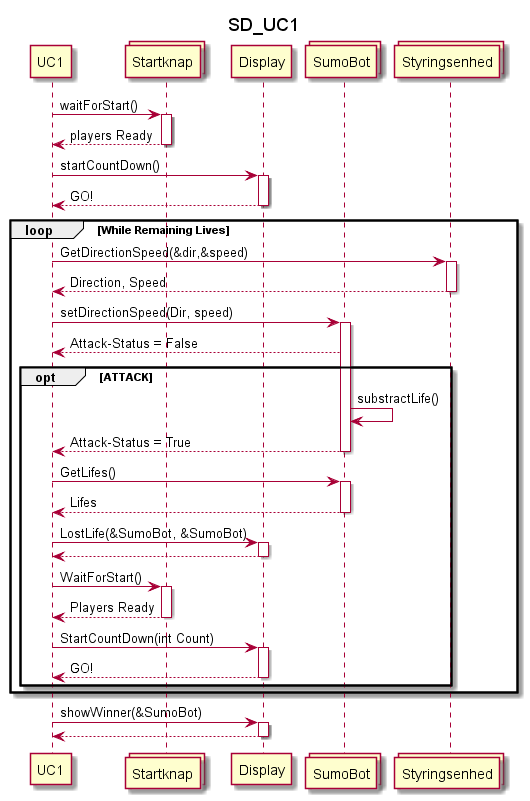
\includegraphics[width=\textwidth]{figs/Design/Central Computer/SekvensDiagrammer/SD_UC1.png}
    \caption{Sekvensdiagram for Central Computer i UC1}
    \label{fig:CC_SD_UC1}
\end{figure}

\subsection{Klassediagram}
På baggrund af sekvens-diagrammets funktioner og funktionskald på tværs af klasser er der udformet et klassediagram med relevante funktioner og relationer, som ses i figur \ref{fig:CC_CD_UC1}. 

\begin{figure}
    \centering
    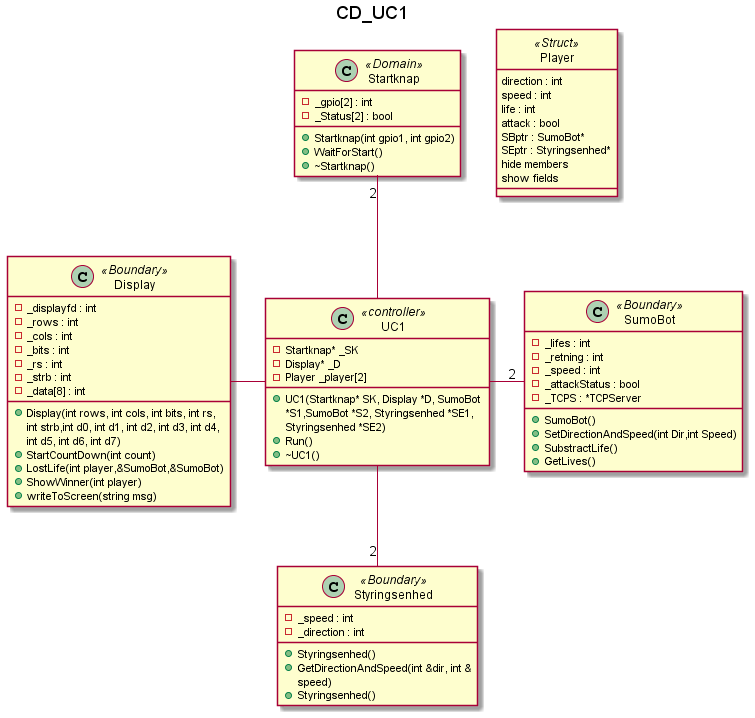
\includegraphics[width=\textwidth]{figs/Design/Central Computer/applikationsmodel/CD_UC1.png}
    \caption{Klassediagram for Central Computer i UC1}
    \label{fig:CC_CD_UC1}
\end{figure}

\subsubsection{Player}
\label{subsubsec:Player}
På klassediagrammet ses også en struktur (struct) kaldet Player, som indeholder vigtig information om hver spiller. Strukturen Player er dannet med henblik på at give mulighed for en implementering hvor loopet afbilledet i sekvensdiagrammet figur \ref{fig:CC_SD_UC1}, "While Remaining Lives" kan blive en løkke som gentager sig for hver spiller, hvis information og pointersså kan ligger gemt i et array - hvert gennemløb af loopet kan så skiftevis være for player ét og 2.Således bliver koden halvt så lang, mere overskuelig og det vil med samme kode blive let at tilføje flere spillere.  

%%%%%%%%%%%%%% Klassen UC1 %%%%%%%%%%%%%%%%%%%

\subsubsection{UC1}
UC1 er controllerklassen \cite{ApplikationsmodellerI2ISE} igennem hvilken use case 1 eksekveres. 
\paragraph{Attributter}
UC1 skal for at kunne benyttes bruge pointers til klasserne Startknap og Display. Derudover skal der for hver spiller også bruges en henvisning til en klasse af typen SumoBot og Styringsenhed - dette gemmes bla. i strukturen Player, som UC1 klassen benytter 2 af. 
\paragraph{Metoder}
I dette afsnit vil klassen UC1's metoder blive beskrevet. 

\begin{functionDescription}
{UC1::UC1(Startknap* SK, Display* D, SumoBot* SB1, SumoBot* SB2, Styringsenhed* SE1, Styringsenhed* SE2)}
{func:UC1_constructor}
{UC1 constructoren sætter den række pointers som nævnt i attributter såvel som liv til at starte på 3. Skriver iøvrigt "Welcome to Robo Sumo Battle" ud på displayet}
{\begin{itemize}
    \item \textbf{Startknapt* SK:} Reference til et Startknap objekt. 
    \item \textbf{Display* D:} Reference til et Display objekt
    \item \textbf{SumoBot* SB1:} Reference til det SumoBot objekt som repræsenterer den SumoBot som skal styres af Player 1
    \item \textbf{SumoBot* SB2:} Reference til det SumoBot objekt som repræsenterer den SumoBot som skal styres af Player 2
    \item \textbf{Styringsenhed* SE1:} Reference til den det Styringsenhed objekt som repræsenterer den styringsenhed som skal Player 1 benytter
    \item \textbf{Styringsenhed* SE2:} Reference til den det Styringsenhed objekt som repræsenterer den styringsenhed som skal Player 2 benytter
\end{itemize}}
{Returnerer et UC1 objekt}
\end{functionDescription}

\begin{functionDescription}
{UC1::Run}
{func:UC1_run}
{Dette er funktionen som eksekverer UC1 med de angivne enheder i constructoren. Funktionens sekvens holder sig stringent til sekvensdiagrammet som ses i figur \ref{fig:CC_SD_UC1}}
{N/A}
{N/A}
\end{functionDescription}

\begin{functionDescription}
{UC1::~UC1()}
{func:destructor_UC1}
{Destructor for UC1 som blot skriver "Goodbye..." ud på skærmen}
{N/A}
{N/A}
\end{functionDescription}

%%%%%%%%%%% Klassen Startknap %%%%%%%%%%%%%%5

\subsection{Startknap}
Klassen Startknap har til formål at interface og interagere med de to startknapper, som fysisk sidder ifm. de to styringsenheder, hvorpå de to spillere kan angive at de er klar til at spille. 

\textbf{Prerequisites:}
Startknap gør brug af biblioteket wiringPi\cite{2020Http://wiringpi.com/}.

\paragraph{Attributter}
Klassen Startknap indeholder en attribut til hhv. at indeholde status for hvorvidt de to respektive spillere har tilkendegivet at de er klar til at starte spillet, på hver deres startknap og en attribut til at indeholde information om hvilken GPIO-port på den embedded controller som startknappen er tilsluttet. 

\begin{functionDescription}
{Startknap::Startknap(int gpio1, int gpio2)}
{func:Startknap_constructor}
{Startknappens constructor initialiserer funktionerne i wiringPi\cite{2020Http://wiringpi.com/}, sætter attributten \textit{gpio} og sætter disse som udgang.
}
{\begin{itemize}
    \item \textbf{int gpio1:} GPIO'en på den embedded controller hvorpå den ene startknap er tilslutte. Bemærk at GPIO nummereringer er foretaget på baggrund af wiringPi bibliotekets nummerering\footnote{http://wiringpi.com/pins/}. 
\end{itemize}}
{N/A}
\end{functionDescription}

\begin{functionDescription}
{void Startknap::waitForStart()}
{func:Startknap_waitForStart}
{Funktionen foretager "busy waiting" indtil begge spillere har tilkendegivet at de er klar til at spille på deres startknap og tager iøvrigt udgangspunkt i at startknapperne er aktivt høje. Funktionen husker tilkendegivningerne således at de to spillere ikke behøver at tilkendegive at de er klar samtidig}
{N/A}
{N/A}
\end{functionDescription}

\begin{functionDescription}
{Startknap::~Startknap()}
{func:Startknap_destructor}
{Klassen Startknap benytter en default destructor da wiringPi's API ikke stiller krav til at skulle frigive GPIO'erne}
{N/A}
{N/A}
\end{functionDescription}

%%%%%%%%%%%%% Klassen Display %%%%%%%%%%%%%%%%%5
\subsection{Display}
Klassen display håndterer kommunikationen på displayet. Klassen er lavet med metoder med prædefinee tekster således at der fra use case klasserne blot skal kaldes eksempelvis én funktion med et heltal, for at vise en nedtælling. En funktion gør brug af hjælpeklassen lcd.h fra biblioteket wiringPi\cite{2020Http://wiringpi.com/}, men har sin egen logik til at flytte cursoren på LCD skærmen såvel og parse strings ud på denne. 

\textbf{Prerequisites:} wiringPi biblioteket fra hvilket der er benyttet metoder til at initialisere GPIOs, flytte LCD-cursoren og overføre enkelte bogstaver.

\paragraph{Attributter}
\begin{itemize}
	\item \textbf{int \_displayfd:} En filedescriptor som fungerer som \textit{handle} til displayet. 
	\item \textbf{int \_rows:} Antallet af rækker som det tilsluttede display har
	\item \textbf{int \_cols:} Antallet af kolonner som det tilsluttede display har
	\item \textbf{int \_bits:} Antallet af bits som bruges til at interface displayet (4 eller 8)
	\item \textbf{int \_rs:} Repræsenterer den GPIO på embedded controller som er forbundet til displayets RS-pin\footnote{Register Select}
	\item \textbf{int \_strb:} Repræsenterer den GPIO på embedded controller som er forbundet til displayets Strobe-pin\footnote{Pin til at opdatere displayet}. 
	\item \textbf{int \_data[8]:} Repræsenterer de 8 GPIO'er på embedded controller som er forbundet til displayets data-pins.
\end{itemize}
\paragraph{Funktion()}

\paragraph{\~Funktion()}
\begin{functionDescription}
{Display::Display(int rows, int cols, int bits, int rs, int strb, int d0, int d1, int d2, int d3, int d4, int d5, int d6, int d7)}
{func:Display_constructor}
{Display klassens constructor initialiserer først og fremmest klassen attributter på baggrund af parametrene. Parmetrene benyttes her også til at initialisere LCD-pins vha. metoder fra wiringPi-biblioteket}
{\textit{Se attributter}}
{N/A}
\end{functionDescription}

\begin{functionDescription}
{int Display::writeToScreen(string msg)}
{func:Display_writeToScreen}
{Denne funktion kaldes som udgangspunkt kun af andre funktioner i klassen og kan ansees som en utiliti-funktion, som klassens resterende metoder kan benytte sig af. Funktionen tager den modtagne streng og indledningsvist validerer hvorvidt den kan være på skærmen. Herefter skiftevis skrives et bogstav ud på skærmen og cursoren flyttes tilsvarende hen over skærmens kolonner og rækker. Hvis cursoren møder et newline-character, gås til næste række og der tjekkes løbende om cursoren prøver at overskride den sidste kolonne i sidste række.}
{\textbf{string msg:} Den streng som ønskes skrevet ud på displayet}
{Der returneres -1 for en tekst der er for lang, -2 for en forsøg på at overskride sidste række's sidste kolonne og 0 for succesfuld udskrift på skærmen}
\end{functionDescription}

\begin{functionDescription}
{void Display::startCountDown(int count)}
{func:Display_startCountDown}
{Funktionen viser en nedtælling på skærmen fra det tal som medsendes som parameter. Funktionen benytter busywait fra Linux' egne biblioteker}
{\textbf{int count:} Tallet i sekunder som der skal tælles ned fra}
{N/A}
\end{functionDescription}

\begin{functionDescription}
{void Display::lostLife(int player, SumoBot *S1, SumoBot *S2)}
{func:Display_lost_life}
{Funktionen udskriver på skærmen at en SumoBot har tabt et liv, hvilken SumoBot der har mistet et liv samt den nuværende stilling. Det bemærkes at metoden bygger på at der kun er to spillere - det vil være muligt at modificere denne til at modtaget et UC-objekt som vha. en get-metode vil kunne formidle adgang til \_player-arrayet hvorfra der vil kunne hentes information om flere SumoBot's liv. I denne iteration vil der for simpliciteten blot kunne vises for 2 spillere. 
}
{\begin{itemize}
    \item \textbf{int player:} Hvilken spiller der har mistet et liv. 
    \item \textbf{SumoBot* S1:} Pointer til det ene SumoBot objekt.
    \item \textbf{SumoBot* S2:} Pointer til det andet SumoBot objekt. 
\end{itemize}}
{N/A}
\end{functionDescription}

% \begin{figure}
%     \centering
%     \includegraphics[width=\textwidth]{}
%     \caption{}
%     \label{fig:}
% \end{figure}

% \subsection{Klasse}
% \paragraph{Attributter}
% \paragraph{Funktion()}
% \paragraph{\~Funktion()}

% \begin{functionDescription}
% {Navn}
% {func:label}
% {Beskrivelse}
% {Parametre}
% {Returværdi}
% \end{functionDescription}
\section{Styringsenhed}\label{sec:Styringsenhed:design}
\subsection{ADC}

Da signalprocesseringen også kan foregå på PSoC 5LP er denne platform et oplagt valg til også at designe styringsenhedens ADC'er i. Herved kan analog til digital konvertering og processering integreres i ét modul. Der ses i figur\tbr \ref{fig} et flowdiagram over den tiltænkte virkemåde for ADC og DSP i styringsenheden. 

Til designet af denne enhed er der som inspiration brugt et bredt udvalg af applikationsnoter fra Cypress Semiconductor som har udviklet PSoC 5LP. Den pågældende er af familien CY8C58xx. Opsætningen og implementeringen af ADC og DSP blokken er gjort i PSoC Creator 4.3. 

Delta Sigma ADC komponenten på PSoC kan enten konfigueres ved firmware eller ved et grafisk interface i PSoC Creator 4.3. Her er det grafiske interface brugt, og i det følgende vil designovervejelserne dokumenteres.

\subsubsection{Analog interfaces}
For at få bedst mulig interface til mikrofonforstærker og filter er der på baggrund af applikationsnoten AN58304, s. 3 \tbr REFERENCE  ... valgt port [P0:7] som indgang til ADC'en, da denne er en af de foreskrevne analoge porte med bedst performance. 

\subsubsection{Input range}
\begin{figure}
    \centering
    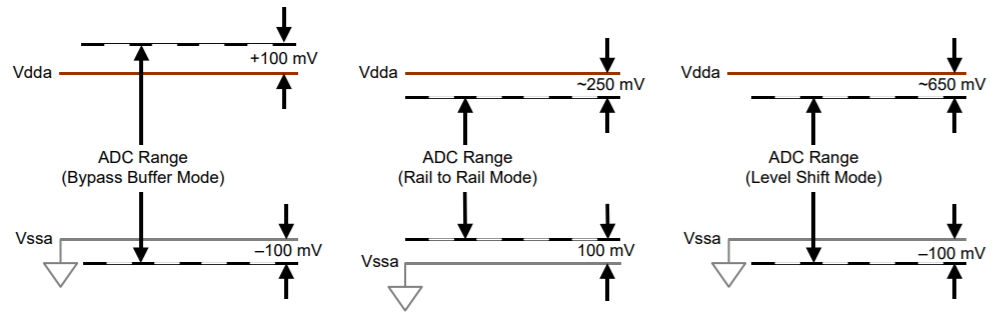
\includegraphics{figs/Design/Styringsenhed/inputrange.PNG}
    \caption{Forskellige input modes for Delta Sigma ADC}
    \label{fig:ADC_inputrange}
\end{figure}
For at få så meget headroom og derved opløsning som muligt, konfigueres ADC'en til (i princippet) rail to rail operation. Men ved denne konfiguration i PSoC aktiveres en buffer på indgangen for at give mulighed for at forstærke indganssignalet. Dette fravælges (bufferen bypasses), for at opnå størst muligt headroom og derved opløsning, se Figur \ref{fig:ADC_inputrange}. Hertil opnås den højest mulige indgangsimpedans,  da anvendelsen af denne buffer er på bekostning af indgangsimpedansen.\tbr REFERENCE TIL DELTA SIGMA ADC, s. 12. Hvis der herved opstår problemer med overstyring af ADC'en, kan der konfigureres til rail-to-rail med buffer gain på 1. 

\subsubsection{Input mode}
\subsubsection{Referencespændinger}
PSoC 5LP har interne referencespændinger med en tolerance på +- 0.1\%. \tbr Reference til datablad for PSoC, side 94.



\subsubsection{Interrupt, polling, DMA}





\subsection{DSP blokken}

\begin{functionDescription}
    {uint8 DoFFT(uint8* inputArray, uint16* FFTResultPtr)}
    {func:DoFFT}
    {Funktionen udregner 128 FFT koefficienter, der efterbefølgende behandles som et styringssignal. }
    {inputArray: Pointer til den samplede ADC data\newline
    FFTResultPTR: Pointer til den de udregnede FFT koefficienter}
    {Ingen}
\end{functionDescription}
\section{SumoBot}\label{sec:SumoBot:design}

\subsection{Overordnet}

Dette afsnit omhandler designet af SumoBotten. Da UC1 og UC2 kun har styringsformen til forskel, skal SumoBotterne udføre samme funktion i begge Use Cases.
Der er i Analysen over SumoBotten blevet udarbejdet nogle specifikke krav, og ud fra disse krav vil der blive fastlagt hvilke komponenter der skal anvendes til konstruktionen af SumoBotterne. 

\subsection{Valg af komponenter}

Ud fra de krav stillet til delblokkene igennem analysen, er der på markedet søgt efter mulige kandidater, der vil kunne efterleve disse krav. Komponentkandidaterne er for overskuelighedens skyld opsat i tabeller. De enkelte komponenter vil for hvert krav blive be- eller afkræftet, for til sidst at få tildelt en "score". Afsluttende vil scoreren for hver komponent blive sammenlignet og på den måde finde den komponent der vil repræsentere systemet bedst muligt.

\subsubsection{Attack Sensor}
\textbf{Krav}
\begin{enumerate}
\item Skal kunne registrere vandret tryk fra sumobot.
\item Skal kunne håndtere 5V med mellem 0 og 20 mA.
\item Skal kunne holde til minimum 10000 tryk.
\end{enumerate}
\begin{center}
\begin{tabular}{|p{2.5cm}||p{1.3cm}|p{1.3cm}|p{1.3cm}|p{1cm}|}
 \hline
 \multicolumn{5}{|c|}{Attack Sensor} \\
 \hline
 Komponent & Krav 1 & Krav 2 & Krav 3 & Score\\
 \hline
 SKHCBJA010 & ja & ja & ja & 3/3\\
 631NH/2 & nej & ja & ja & 2/3\\
 \hline
\end{tabular}
\end{center}
\textbf{Valg}
De to komponenter der har stået til overvejelse, har henholdsvis fået scoreren 3/3 og 2/3 jævnfør deres respektive datablade. På baggrund at dette, er det blevet konkluderet, at valget til projektet ligger på SKHCBJA010. Denne sensor kan håndtere kontakt fra alle sider, kan lede strømme på over 20 mA og ligeledes tolerer flere tusinde påvirkninger inden fejl. Selve implementering og montering kan findes i afsnit xx.

\subsubsection{PSU}
\textbf{Krav}
\begin{enumerate}
\item Skal kunne levere en stabil 5V DC forsyning  med maks afvigelse på  4.80 < 5.00 < 5.20 V ved 25 grader.
\item Skal kunne lervare minimum 500 mA.
\item Skal kunne køre stabilt med et 7 til 12V DC input.
\item Skal kunne videresende Batteri forsyningen.
\item Må ikke fylde mere end 4x4x4 cm
\item Må maks have en output noice voltage på 120 mikroVolt
\end{enumerate}
\begin{center}
\begin{tabular}{|p{2.5cm}||p{1.3cm}|p{1.3cm}|p{1.3cm}|p{1.3cm}| p{1.3cm}| p{1.3cm}| p{1cm}|}
 \hline
 \multicolumn{8}{|c|}{PSU} \\
 \hline
 Komponent & Krav 1 & Krav 2 & Krav 3 & Krav 4 & Krav 5 & Krav 6 & Score \\
 \hline
 MC7805B & ja & nej & ja & ja & ja & ja & 5/6\\
 LM7805 & ja & ja & ja & ja & ja & ja & 6/6\\
 \hline
\end{tabular}
\end{center}
\textbf{Valg}

Ud fra ovenstående tabel kan der konkluderes at "pas" er den rette komponent at anvende i projektet, da denne opfylder alle vores komponentkrav.  


\subsubsection{Mikrocontroller}
\textbf{Krav}
\begin{enumerate}
\item Skal kunne kommunikere  over WIFI.
\item Skal have minimum 10 In/Out ben.
\item Skal kunne køre 5V DC.
\item Skal kunne levere mellem 3.3V og 5V DC på output benene.
\item Må Maks være 12x4x4 cm.
\end{enumerate}
\begin{center}
\begin{tabular}{|p{3.5cm}||p{1.3cm}|p{1.3cm}|p{1.3cm}| p{1.3cm}| p{1.3cm}| p{1cm}|}
 \hline
 \multicolumn{7}{|c|}{Microcontroller} \\
 \hline
 Komponent & Krav 1 & Krav 2 & Krav 3 & Krav 4 & Krav 5 & Skore \\
 \hline
 Arduino mega 2560 & ja & nej & ja & ja & ja & 4/5\\
 Raspberry Pie Zero & ja & ja & ja & ja & ja & 5/5\\
 raspberry pie 4 & ja & ja & ja & ja & ja & 5/5\\
 \hline
\end{tabular}
\end{center}
\textbf{Valg}

Som brugbar mikrocontroller til projektet, har ovenstående 3 controllere være til overvejelse. 
Ud fra ovenstående tabel kan der konkluderes at "pas" er den rette komponent at anvende i projektet, da denne opfylder alle vores komponentkrav.  


\subsubsection{Motor}
\textbf{Krav}
\begin{enumerate}
\item Skal have et moment på minimum 0.526 kg-cm.
\item Skal være en DC motor.
\item Må maksimalt være være 8x4x4 cm med akse.
\end{enumerate}
\begin{center}
\begin{tabular}{|p{2.6cm}||p{1.3cm}|p{1.3cm}|p{1.3cm}|p{1cm}|}
 \hline
 \multicolumn{5}{|c|}{Motor} \\
 \hline
 Komponent & Krav 1 & Krav 2 & Krav 3 & Skore\\
 \hline
  238-9715 & nej & ja & ja & 2/3\\
 F280 Planet gear & ja & ja & ja & 3/3\\
 \hline
\end{tabular}
\end{center}
\textbf{Valg}

Ud fra ovenstående tabel kan der konkluderes at "pas" er den rette komponent at anvende i projektet, da denne opfylder alle vores komponentkrav. 

\subsubsection{Motorstyring}
\textbf{Krav}
\begin{enumerate}
\item Skal kunne anvende 5V logik.
\item Skal kunne anvende 3.3V på input/PWM indgangene.
\item skal kunne styre retning og hastighed på 2 motorer uafhængigt af hinanden.
\item Skal kunne styre hastighed ved hjælp af PWM.
\item Skal kunne håndtere minimum 2A load kontinuerligt ved minimum 12V DC.
\item Skal kunne klare 12V DC indgang / udgang. 
\item Må ikke være større end 5x5x5 cm
\end{enumerate}
\begin{center}
\begin{tabular}{|p{2.1cm}||p{1.3cm}|p{1.3cm} |p{1.3cm} |p{1.3cm}|p{1.3cm}| p{1.3cm}| p{1.3cm}| p{1cm}|}
 \hline
 \multicolumn{9}{|c|}{Motorstyring} \\
 \hline
 Komponent & Krav 1 & Krav 2 & Krav 3 & Krav 4 & Krav 5  & Krav 6 & Krav 7 & Skore \\
 \hline
 L293D  & ja & ja & ja & ja & nej & ja & ja & 6/7\\
 L298n & ja & ja & ja & ja & ja & ja & ja & 7/7\\
 \hline
\end{tabular}
\end{center}
\textbf{Valg}

Ud fra ovenstående tabel kan der konkluderes at "pas" er den rette komponent at anvende i projektet, da denne opfylder alle vores komponentkrav.  

\subsection{DOmænemodel for UC1 og UC2}

\subsubsection{Sekvensdiagram}
\subsubsection{Klassediagram}

\subsection{Software}



%% Implementering !
\chapter{Implementering}

\include{TeX/Implementering/SumoBot_Implementering}

%% Litteraturliste
\addcontentsline{toc}{chapter}{Litteraturliste}
\bibliographystyle{IEEEtran}
\bibliography{biblo}

\clearpage

%%% Bilag
\addcontentsline{toc}{chapter}{Bilag}
\appendices
\chapter{Revisionshistorik}

% Revisionshistorik
\begin{table}[!h]
    \centering
    \begin{tabular}{lllp{5cm}}
        \textbf{Revision} & \textbf{Dato} & \textbf{Forfatter} & \textbf{Beskrivelse} \\
        2.0               & 2020-11-27    & AH DS           & Joystick fjernes fra systemet. Styringsenhedens input er genanalyseret og revideret deraf. \\
        1.0               & 2020-11-11    & RK                 & Revisionshistorik tilføjet\\
    \end{tabular}
\end{table}

\end{document}
